\documentclass[output=paper]{langscibook} 
\ChapterDOI{10.5281/zenodo.5675845}
\author{Björn Wiemer\affiliation{Johannes Gutenberg Universität Mainz}}
\title[No paradigms without classification]{No paradigms without classification: How stem-derivation develops into grammatical aspect}
\abstract{The Slavic aspect (pfv.:ipfv.) system is based on a binary opposition of stems connected by derivational patterns. The choice between pfv. and ipfv. stem is unavoidable, since it affects virtually any finite and non-finite form. Simultaneously, this opposition is characterized by classificatory properties resulting from complementary inventories of heterogeneous functions and constraints assigned to pfv. and ipfv. stems, respectively. This situation raises questions as for the paradigmatic organization of lexical units represented by verb stems, and an argument is developed for a two-layer structure of paradigms which integrates the crucial role played by complementary inventories of functions and constraints associated to ipfv. vs pfv. stems. Concomitantly, a case is made for a moderate paradigm-based model of morphology in which stems are the basic units. On this background also Construction Grammar approaches to grammatical categories are evaluated and useful parallels to Word-and-Paradigm models are elaborated on to show which hitherto unnoticed profit can be gained for a theory of grammatical oppositions by a due account of the properties of the Slavic aspect system.}


\begin{document}
\maketitle 

\section{Introduction}\label{wiemer:1}

The opposition of perfective (pfv.) : imperfective (ipfv.) aspect is a kind of “proprietary label” of Slavic languages as a whole. The fundamental architecture of this system is the same for all varieties of Slavic, both concerning the morphological patterns and the basic functional distinctions (see \sectref{wiemer:2}). The pfv.:ipfv. opposition is binary, and the backbone of the system are regular and predictable patterns of stem-derivation (\sectref{wiemer:2.1}). As a consequence, practically every finite and non-finite form of a verb belongs to either pfv. or ipfv. aspect. This makes aspect choice almost unavoidable, and since verbs play a central role in syntax and participate in many categorial distinctions, aspect choice bears severe consequences for the grammatical system of any Slavic language. Simultaneously, the distribution of pfv. and ipfv. stems over contexts that can be defined by grammatical or pragmatic conditions raises questions about the lexical units on which aspect operates, and about the paradigmatic organization of verb stems representing such units (\sectref{wiemer:2.2}). This is why the history of Slavic aspectology abounds in discussions concerning the morphological status of the pfv.:ipfv. opposition and its interaction with the lexicon. Central to this discussion are countless debates as for which ipfv. and pfv. stems represent the same lexical meaning (so that they can be considered pairs, partners or groups) and how these relations should be captured in systematic lexicography, but also how the paradigmatic structure of morphologically related verb stems of opposite aspect may be captured (see \sectref{wiemer:3}).

These traditional debates, in particular the issue of paradigmatic organization, are here re-evaluated: by choosing a stem, one chooses aspect, and this choice correlates with various grammatical constraints and functional oppositions, largely depending on different types of construction. The choice therefore depends on sets of functions and constraints, and these sets lean  toward complementary distribution over two classes of stems, called perfective and imperfective. Aspectual distinctions belong to the core functions influencing this choice, but many more oppositions and constraints have appeared since the onset of a development by which diverse kinds of contextual implicatures have been strengthened and entrenched via the choice of stems. These stems organize into two classes (class of pfv. stems vs class of ipfv. stems) and thus make up a binary classificatory system.

\citet[125]{Plungjan2000} defines classificatory categories as follows:

\begin{quote}
[1] (…) a given amount of lexemes of a language distributes over non-over\-lap\-ping subclasses without any remainder; every subclass is characterized by its meaning for a certain grammatical category. Therefore, this category is assigned not to word forms, but to lexemes and determines the grammatical \textit{classification} of the [given section of the] lexicon. This is why it is called classificatory.\\\hbox{}\hfill (my translation, emphasis original; see also \citealt[53--54]{Plungjan2011})\hbox{}
\end{quote}

\noindent Plungjan considers Slavic aspect a prominent example of a classificatory category. Accepting this, I further argue that the units underlying grammatical classification are stems and that, first of all, the grammatical classes (inventories of pfv. stems vs ipfv. stems) are themselves established and strengthened by an increasing amount of very heterogeneous functions and constraints in complementary distribution. Thus, complementary inventories and the binary opposition of two increasingly abstract classes condition each other mutually (see \sectref{wiemer:2.2}).

From these premises, I arrive at two interrelated claims which will be argued for in this article, namely

\begin{description}\sloppy
\item[Claim 1:]  The tight organization of complex paradigmatic oppositions conditioned by aspect choice in Slavic (the pfv.:ipfv. opposition), though based on stem-derivation, can only be explained from the classificatory properties of the system; these properties, in turn, result from the formation of complementary sets of functional (grammatical and pragmatic) oppositions and constraints.
\item[Claim 2:]   The complementary sets participate in the formation of a complex paradigmatic system, “on top” of traditional sets of finite and non-finite verb forms; the nature and provenance of this paradigmatic organization considerably modifies known conceptions of paradigms.
\end{description}

Concomitantly, these properties explain why the rise of the Slavic aspect opposition is no good example of grammaticalization. Among standard parameters, as those in \citet{Lehmann1995, HeineKuteva2002, Himmelmann2004}, only paradigmatic tightening and, to a much smaller extent, syntagmatic tightening apply, in a sense context expansion can be considered as well, but other parameters are practically irrelevant, or useless \parencites[Ch. 6]{Wiemer2002}{Wiemer2008}[267--270]{Wiemer2020a}{WiemerSerzant2017}. This said, I have to specify in which sense paradigmatic and syntagmatic tightening as well as context expansion apply and why the rise of tighter paradigmatic relations is crucial for an understanding of this grammatical opposition. The question whether the related processes and their results may be subsumed under grammaticalization is tangential to (and unrevealing for) a proper explanation of how this opposition works and how its paradigmatic organization looks like. More so, I dare claim that neither Construction Grammar nor Word-and-Paradigm approaches, as known so far, are able to provide a fully adequate description (let alone explanation), although it is certainly among these approaches where we have to look for an adequate model.

This sets the stage for the following. I will start with the essentials about the Slavic pfv.:ipfv. opposition; this presentation glosses over many details, is far from comprehensive and refrains from giving a diachronic background. It is restricted to what is necessary to justify why aspect in contemporary Slavic should be considered a classificatory system based on stem derivation (\sectref{wiemer:2}), and what is indispensible for a proper understanding of the problematic relation between paradigm and lexeme, which will be addressed in \sectref{wiemer:3}. Subsequently, I will discuss the merits and limits of Construction Grammar approaches and Word-and-Paradigm models for an account of the architecture of aspect in Slavic (\sectref{wiemer:4}), before I address my own proposal of an extended notion of paradigm applied to aspect choice (\sectref{wiemer:5}). The article ends with a summary and an outlook (\sectref{wiemer:6}).

Two “technical” remarks should be added: if no elaborate glossing is needed, I will indicate the aspect of the stem by upper case small caps (\textsc{\textsuperscript{ipfv}}, \textsc{\textsuperscript{pfv}}), and examples given without an indication of their source are constructed.

\section{The basic architecture of the Slavic pfv.:ipfv. opposition} \label{wiemer:2}


Essentially, the pfv.:ipfv. opposition of Slavic languages rests on two pillars, one consists in patterns of morphological derivation (\sectref{wiemer:2.1}), the other in the distribution of verb stems over (a) function inventories and (b) sets of combinatorial restrictions (\sectref{wiemer:2.2}). Both pillars provide the foundation for paradigmatic oppositions and render them grammatical, but while the first pillar assigns some regularity of form to this opposition, it is the distributional properties of the involved stems which turn it into a classificatory category. These two characteristics – patterns of stem derivation and grammatical classification – are not only compatible, by capturing different properties of Slavic aspect \citep{Wiemer2006}, but depend on one another; moreover, they justify the combination of different models of morphological analysis. Among these, Word-and-Paradigm approaches are more important.

\subsection{Stem-derivational patterns} \label{wiemer:2.1}

In Slavic, aspect is not indicated by unequivocal, monofunctional morphemes. Instead, the morphology of aspect builds on the functional reinterpretation of patterns of stem derivation which uses both prefixes and suffixes (\citealt{Breu2000, Wiemer2008, WiemerSerzant2017}, among many others). Apart from minor, often lexically restricted and obsolete patterns, two patterns predominate and are productive across contemporary Slavic; see \figref{fig:wiemer:predom} with infinitives.

\begin{figure}
  \caption{Predominant patterns of stem derivation and their grammatical reinterpretation\label{fig:wiemer:predom}}
  \begin{tikzpicture}
  \matrix (matrix) [matrix of nodes, nodes={anchor=base west}] 
    {
     a. & simplex  & ${\Rightarrow}$ &  \textsc{prefix}+simplex\\
     b. &          &                 &   prefixed stem ${\Rightarrow}$  [prefixed stem]+\textsc{suffix}\\[2cm]
     c. & simplex\textsc{\textsuperscript{ipfv}} & --- &  prefixed stem\textsc{\textsuperscript{pfv}}\\[-4pt]
      &                                        &     &  (e.g., Pol. \textit{gotowa-ć} ${\Rightarrow}$ \textbf{\textit{u}}\textit{-gotowa-ć} ‘cook’)\\
     d. &                                      &     & prefixed stem\textsc{\textsuperscript{pfv}} --- [[prefixed stem]+\textsc{suffix}]\textsc{\textsuperscript{ipfv}}\\[-4pt]
      &                                        &     & (e.g., Pol.\textit{prze-kaza-ć} ${\Rightarrow}$ \textit{prze-kaz-}\textbf{\textit{ywa}}\textit{{}-ć} ‘convey’;\\[-4pt]
      &                                        &     & \textit{s-praw-i-ć} ${\Rightarrow}$ \textit{s-prawi-}\textbf{\textit{a}}\textit{{}-ć} ‘cause’)\\
    };
   \coordinate [right=1cm of matrix-2-4.south west] (anchor-1);
   \draw[-{Implies[]}, double, semithick] (anchor-1) -- ++ (0,-2cm) node [midway, right] {\begin{tabular}{@{}l@{~}l@{}}
                                                                                                   reinterpretation: & (a) identical lexical concept\\
                                                                                                                     & (b) different gram. distribution
                                                                                                \end{tabular}};
  \end{tikzpicture}  
\end{figure}      

Importantly, markers of tense, mood, agreement (person/number) and of non-finite forms all occur outside of these stems. Although such ending sets are associated with systematic morphonological alternations, e.g., between present (resp. non-past) and infinitive stems, these alternations apply to any stem regardless of its aspect. This predictably leads to multiple exponence, e.g. the non-past and the infinitive stem each imply particular sets of endings (see \ref{ex:wiemer:3}a--b), so do allomorphs of imperfectivizing suffixes, like -\textit{ywa}{}- vs -\textit{uj}{}- in Polish (see \ref{ex:wiemer:4}--c). Thus, the patterns of stem changes that distinguish aspect are entirely dissociated from alternations between non-past and infinitive stems, i.e. from what \citet[199]{Brown1998} dubs ``allostems''. These two types of stem change are not related diachronically, and despite regular morphonological alternations at the end of stems (or: before endings), the word-form structure shows clear morpheme boundaries;\footnote{There also occur language-specific regular changes in the root vowel (apophony), e.g. Pol. \textit{przepowi}\textrm{\textbf{\textit{e}}}\textrm{\textit{dzieć}}\textrm{\textsc{\textsuperscript{pfv}}} \textit{– przepowi}\textrm{\textbf{\textit{a}}}\textrm{\textit{dać}}\textrm{\textsc{\textsuperscript{ipfv}}} \textrm{‘forecast.}\textsc{inf}’, but these non-concatenative alternations are likewise irrelevant for aspect membership. They can supply additional cues for its recognition, but never independently from the patterns given in \figref{fig:wiemer:predom}, and from multiple prefixation if it applies (see below).} in this respect, it follows concatenative principles: typically, portmanteau morphemes are known for material added on stems, not of stems themselves. See (\ref{ex:wiemer:3}--\ref{ex:wiemer:4}) from Polish, where square brackets indicate the part of the word forms which constitutes the stem relevant for determining aspect. They show the word form structure and non-aspect related stem-alternations in the derivation of perfective and imperfective stems with finite past and non-past forms.

% ex. 3+4 were fig. 2 before 
\ea \label{ex:wiemer:3} 
{[1] Simplex imperfective stem ${\Rightarrow}$ perfective stem by prefixation}\\
\ea \label{ex:wiemer:3a}\begin{minipage}[t]{\widthof{‘she wrote, was writing’~~~}}
    \gll [{pis-a}]\textsc{\textsuperscript{ipfv}}{{}-ł-a}\\ 
         write-\textsc{thv-pst-sg.f}\\                                    
    \glt ‘she wrote, was writing’\end{minipage}  ${\Rightarrow}$ \hspace{1ex}
    \begin{minipage}[t]{.4\linewidth}
    \gll [{na-pis-a}]\textsc{\textsuperscript{pfv}}{-ł-a} \\
              \textsc{pfx}{}-write-\textsc{thv-pst-sg.f}\\                
     \glt ‘she wrote (up)’\end{minipage}          
\ex \label{ex:wiemer:3b}\begin{minipage}[t]{\widthof{‘I write, am writing’~~~~}}
    \gll  [{pisz}]\textsc{\textsuperscript{ipfv}}{{}-ę}\\                         
    write.\textsc{prs-prs.1sg} \hphantom{text}\\                                                
    \glt     ‘I write, am writing’\end{minipage} ${\Rightarrow}$  \hspace{1ex}                
    \begin{minipage}[t]{\widthof{\textsc{pfx}{}-write.\textsc{prs-prs.1sg}~~}}   
    \gll [{na-pisz}]\textsc{\textsuperscript{pfv}}{{}-ę} \\ 
         \textsc{pfx}{}-write.\textsc{prs-prs.1sg}\\
  \glt ‘I will write (up)’\\ \end{minipage}  (< *{(na-)pis-jǫ})                                                 
\z \ex \label{ex:wiemer:4} 
{[2] Perfective stem by prefixation ${\Rightarrow}$  secondary imperfective stem by suffixation}\\
 \ea \label{ex:wiemer:4a}\begin{minipage}[t]{.4\textwidth}
\gll [{roz-wiąz-a}]\textsc{\textsuperscript{pfv}}{{}-l-i}\\         
     \textsc{pfx}{}-bind-\textsc{thv-pst.vir-pl.vir}\\           
\glt    ‘they tied off’    \end{minipage} ,  \hspace{1ex} 
\begin{minipage}[t]{.4\textwidth}
\gll [{roz-wiąz-a}]\textsc{\textsuperscript{pfv}}{{}-ć}\\
     \textsc{pfx}{}-bind-\textsc{thv-inf}\\
\glt  ‘tie off’ \\
\end{minipage}
 \ex \label{ex:wiemer:4b}
  ${\Rightarrow}$ \begin{minipage}[t]{.366\textwidth}
  \gll [{roz-wiąz-ywa}]\textsc{\textsuperscript{ipfv}}{{}-l-i}\\   
   \textsc{pfx}{}-bind-\textsc{sfx-pst.vir-pl.vir}\\
   \glt     ‘they tied off, were tying off’
   \end{minipage} , \hspace{1ex} \begin{minipage}[t]{.35\textwidth}
 \gll  [{roz-wiąz-ywa}]\textsc{\textsuperscript{ipfv}}{{}-ć}\\
       \textsc{pfx}{}-bind-\textsc{sfx-inf}\\
 \glt ‘tie off’\\
 \end{minipage}
 \ex \label{ex:wiemer:4c}
 \gll [{roz-wiąz-uj}]\textsc{\textsuperscript{ipfv}}{{}-ą}\\
    \textsc{pfx}{}-bind-\textsc{sfx-prs.3pl}\\
  \glt   ‘they tie, are tying off’\\
 \z\z


This standard segmentation of word forms into morphemes, with an account of allomorphy, looks like an application of an Item-and-Process (IP) analysis, inasmuch as morphonological changes are accounted for, or even an Item-and-Arrangement (IA) analysis, inasmuch as merely  concatenative principles are considered. However, such analyses miss the crucial point that these allomorphic alternations are accidental, and thus irrelevant for determining the membership of the stem to pfv. or ipfv. aspect. It is not the affixes themselves which determine aspect but patterns standing in opposition to another stem which is formally distinguished by presence vs lack of a prefix or suffix.\footnote{Here I am neglecting differences between addition and change (or alternation) of suffixes, for reasons that become clear in Sections~\ref{wiemer:2.2} and~\ref{wiemer:3}.} Since these stem distinctions apply “before” markers of tense and agreement are added, each stem already distinguished as pfv. or ipfv. can have all kinds of finite and non-finite forms, or conversely: aspect is in principle distinguished for all finite and non-finite forms (infinitive, participles, action noun); cf. also \textcitetv{chapters/02_andersen}.

As the patterns in \figref{fig:wiemer:predom} and (\ref{ex:wiemer:3}--\ref{ex:wiemer:4}) show, the locus of the affix is also crucial: most simplex stems are ipfv., while prefixation almost always yields a pfv. stem, and the addition (or change) of another suffix makes an already prefixed stem ipfv. While the latter, i.e. so-called secondary imperfectivization, almost never changes the lexical meaning of the stem, prefixes normally change it. In those cases, the prefix serves both a lexical function (it changes lexical meaning and thereby partakes in creating a new lexical unit) and a grammatical function (it changes an ipfv. stem into a pfv. one).

In contrast to prefixes, the number of suffixes used in secondary imperfectivization (see \ref{ex:wiemer:4b}) is much smaller, in fact contemporary Slavic languages tend to have only one productive suffix, such as Russ./Pol./Cr. \{iva\}, Czech \{ova\}, Bulg.\slash Bel. \{va\}. It has as such become a salient sign of imperfectivization which, above all, does not change lexical meaning. For this reason, many have regarded it as a grammatical marker of ipfv. aspect par excellence. Moreover, because of its productivity secondary imperfectivization has also been viewed as inflection, while other patterns of stem derivation would be ascribed a different grammatical status – with the consequence that Russian aspect has sometimes been treated as a morphologically mixed category. Without going too deeply into this recently revived debate (cf. \citealt{Gorbova2015}), I here only want to point out that nothing in the morphological structure of verb stems forces us to assume that the addition or alternation of suffixes which precede morphemes marking agreement categories (person/number) or tense should be considered as inflection, even if they do not affect lexical meaning and are very productive. Ultimately, the discussion boils down to the question of what counts as a lexical unit and whether these units can be integrated in paradigms (see \sectref{wiemer:3}).

Importantly, aspect membership (i.e. the grammatical function) cannot be explained by derivation as such. Instead, it results from distributional restrictions which do not hinge on pairs of pfv. and ipfv. stems united by an identical lexical meaning, although such pairs constitute a central and necessary part of the system (see \sectref{wiemer:2.2}). By a similar token, aspect assignment does not depend on (a)telicity or actionality features. These tenets will be briefly explained in the remainder of this subsection.

To start with, although the dual – lexical and grammatical – function is characteristic for prefixes added to simplex (predominantly ipfv.) stems, there is a considerable number of cases in which the prefix only marks change of aspect, but does not alter the lexical meaning of the initial ipfv. stem (henceforth: simplex ipfv. = IPFV1). These cases are called Natural Perfectives, following \citet{JandaEtAl2013}: The perfectivizing prefix has a meaning profile which makes it compatible with a component of the lexical meaning of the simplex stem. This results in semantic overlap, so that the lexical meaning remains unaltered. Standard examples are Russ. \textit{pisat’}\textsc{\textsuperscript{ipfv}} ${\Rightarrow}$ \textit{na-pisat’}\textsc{\textsuperscript{pfv}} ‘write’, \textit{stroit’}\textsc{\textsuperscript{ipfv}} ${\Rightarrow}$ \textit{po-stroit’}\textsc{\textsuperscript{pfv}} ‘build’, \textit{pit’}\textsc{\textsuperscript{ipfv}} ${\Rightarrow}$ \textit{vy-pit’}\textsc{\textsuperscript{pfv}} ‘drink’, \textit{čitat’}\textsc{\textsuperscript{ipfv}} ${\Rightarrow}$ \textit{pro-čitat’}\textsc{\textsuperscript{pfv}} ‘read’. Notably, there are no prefixes “specializing” as such in Natural Perfectives (NatPerfs).\footnote{The number of NatPerfs can only be estimated roughly, but they are not a marginal phenomenon. \citet{Łaziński2020}  counted about 1,670 NatPerfs in Polish, which amounts to approx. 36\% of all aspect pairs acknowledged in authoritative dictionaries. For similar figures concerning Russian cf. \citet{JandaEtAl2013}, who emphasize that, on average, the token frequency of NatPerfs exceeds that of pfv. stems with prefixes that modify the lexical meaning of the simplex about 10 times.} NatPerfs are only claimed for telic stems (resp. their telic uses); in atelic contexts, usually the prefix \textit{po}{}- is encountered, which while also perfectivizing, does not mark an action as accomplished, but only as limited in time. Thus, one also gets \textit{pisat’}\textsc{\textsuperscript{ipfv}} ${\Rightarrow}$ \textit{po-pisat’}\textsc{\textsuperscript{pfv}} ‘write’, \textit{pit’}\textsc{\textsuperscript{ipfv}} ${\Rightarrow}$ \textit{po-pit’}\textsc{\textsuperscript{pfv}} ‘drink’, \textit{čitat’}\textsc{\textsuperscript{ipfv}} ${\Rightarrow}$ \textit{po-čitat’}\textsc{\textsuperscript{pfv}} ‘read’ (together with inherently atelic stems like \textit{sidet’}\textsc{\textsuperscript{ipfv}} ${\Rightarrow}$ \textit{po-sidet’}\textsc{\textsuperscript{pfv}} ‘sit’, \textit{kričat’}\textsc{\textsuperscript{ipfv}} ${\Rightarrow}$ \textit{po-kričat}\textsc{\textsuperscript{ipfv}} ‘shout’), while \textit{po-stroit’}\textsc{\textsuperscript{pfv}} ‘build’ is telic simply because \textit{stroit’}\textsc{\textsuperscript{ipfv}} is incapable of atelic readings. This evidences that, regardless of whether telicity is analyzed as a feature of verb (better: stem) semantics or of clause semantics, it is not a defining property of aspect.\footnote{By the same token, perfective aspect only has the function of limiting the situation denoted by the verb; it per se does not mark completion (or similar notions). The latter is possible only with telic predicates.} Instead, the stem-derivational patterns discussed here are grammatical, among other things, because they are not restricted by telicity. Pairs of atelic simplex\textsc{\textsuperscript{ipfv}}—prefixed\textsc{\textsuperscript{pfv}} stems are numerous and can be productively derived (at least in Russian and many other Slavic languages).

Moreover, there are many verbs which denote punctual events and are, in this respect, related to limited events. These demonstrate systematic pairings of pfv. and ipfv. stems (in either direction of morphological derivation) in which the ipfv. stem simply denotes the same event as the pfv. one without any shifts in actionality. Consider, for instance, Russ. \textit{spotk-nu-t’-sja}\textsc{\textsuperscript{pfv}} – \textit{spotyk-a-t’-sja}\textsc{\textsuperscript{ipfv}} ‘stumble’, \textit{lop-nu-t’}\textsc{\textsuperscript{pfv}} – \textit{lop-a-t’-sja}\textsc{\textsuperscript{ipfv}} ‘pop’, verbs denoting illocutionary acts (Russ. \textit{prosit’}\textsc{\textsuperscript{ipfv}} \textit{– po-prosit’}\textsc{\textsuperscript{pfv}} ‘request’, \textit{zajav-i-t’}\textsc{\textsuperscript{pfv}} \textit{– zajavlj-a-t’}\textsc{\textsuperscript{ipfv}} ‘declare’), verbs denoting mental or social events (Russ. \textit{zamet-i-t’}\textsc{\textsuperscript{pfv}} \textit{– zameč-a-t’}\textsc{\textsuperscript{ipfv}} ‘notice, spot’, \textit{prost-i-t’}\textsc{\textsuperscript{pfv}} \textit{– prošč-a-t’}\textsc{\textsuperscript{ipfv}} ‘forgive’). The ipfv. stems only “copy” the event meaning of the pfv. stem, but their function in the grammatical system is important, as they serve to replace their pfv. counterparts in contexts for which the latter are avoided or altogether inadmissible (see \sectref{wiemer:2.2}). In sum, regardless of the actionality type and differences in actional behavior on the clause level, stem derivation changing the grammatical behavior is pervasive and able to “overwrite” differences of actionality types and actional shifts between the related stems.

Two more phenomena are to be mentioned here because they are widespread and, though complicating the system on first sight, on closer inspection they substantially support the generalization that aspect membership is indicated not by particular prefixes (or suffixes), but based on derivational patterns of verb stems which lead to a binary division of stems into grammatical classes. The first “complication” arises with prefixed stems that are able to occur in a double relationship with ipfv. stems. For instance, Russ. \textit{raz-delit’}\textsc{\textsuperscript{pfv}} can be considered the pfv. counterpart to \textit{delit’}\textsc{\textsuperscript{ipfv1}} in the sense of ‘divide, separate’ (= NatPerf), but it also occurs as the pfv. stem to the secondary imperfective (= IPFV2) \textit{raz-delj-a-t}\textsc{\textsuperscript{ipfv2}} in the sense of ‘share (somebody’s opinion)’. The same applies to the Polish cognates \textit{dzielić}\textsc{\textsuperscript{ipfv1}} ${\Rightarrow}$ \textit{po-dzielić}\textsc{\textsuperscript{pfv}} ‘divide, separate’ (= NatPerf) vs \textit{po-dzielić}\textsc{\textsuperscript{pfv}} ${\Rightarrow}$ \textit{podziel-a-ć}\textsc{\textsuperscript{ipfv2}} ‘share (somebody’s opinion, fate)’. In these cases the two different pairs (IPFV1—PFV vs PFV—IPFV2) represent different lexical meanings. However, in many other cases the relation of IPFV1—PFV—IPFV2 establishes so-called aspect triplets: both ipfv. stems can provide “copies” of the lexical meaning of the pfv. stem, while each of them is subject to different constraints and function preferences assigned to ipfv. stems in their entirety (see \sectref{wiemer:2.2}). The pfv. stem, in turn, functions like a pivot, since it connects the two ipfv. stems in a derivational chain; compare:

\ea \label{ex:wiemer:ab}Russian\smallskip\\
       \begin{tabular}[t]{@{} l@{~~}lclcll @{}}
           & IPFV                &               &  PFV                                        &               & IPFV2\\
        a. & {že-č’}      & $\Rightarrow$ & \textit{{s}}{{}-že-č’}        & $\Rightarrow$ & {s-žig-}\textit{{a}}{{}-t’} & ‘burn (\textsc{tr})’\\
        b. & {množ-i-t’}  & $\Rightarrow$ & \textit{{u}}{{}-množ-i-t’}    & $\Rightarrow$ & {u-množ-}\textit{{a}}{{}-t’} & ‘multiply’\\
        c. & {gotov-i-t’} & $\Rightarrow$ & \textit{{pri}}{{}-gotov-i-t’} & $\Rightarrow$ & {pri-gotavl-}\textit{{iva}}{{}-t’} & ‘cook’\\
        \end{tabular}
\z

Such triplets depend, of course, on NatPerfs, and they are even more difficult to count than NatPerfs (see fn. 3). Preliminarily, even in conservative counts\footnote{For a survey of the criteria which have been employed to subdivide aspect triplets cf. \citet[51--56]{Wiemer2019}.} the number of triplets amounts to considerably more than 500 in contemporary Russian, Polish and Czech (\citealt[§3.2]{WiemerEtAlForthc}).

Another pervasive kind of triplet is based on atelic IPFV1 stems denoting unbounded activities consisting of rapid cyclic acts (e.g., ‘wave’, ‘shiver’, ‘blinker’, ‘knock’). They derive two different pfv. stems, one with the prefix \textit{po}{}- adding a temporal limit, the other with a nasal suffix (e.g. Russ. -\textit{nu}{}-) denoting a single act out of the cyclic repetition (semelfactives). Compare:\largerpage[-1] 

\ea \label{ex:wiemer:5}Russian\\
    \ea \begin{tabular}[t]{@{} lcl @{}}
         IPFV &  & PFV\\
          {mig-a-t'}    & $\Rightarrow$ &{\textit{po}-mig-a-t'} \\
         \multicolumn{1}{c}{$\Downarrow$} \\
         PFV\\
         {mig-\textit{nu}-t'}\\
         `blinker'
         \end{tabular}
    \ex \begin{tabular}[t]{@{} lcl @{}}
         IPFV &  & PFV\\
         {vilj-a-t'}     & $\Rightarrow$ & {\textit{po}-vilj-a-t'}\\
         \multicolumn{1}{c}{$\Downarrow$} \\
         PFV\\
         {vil'-\textit{nu}-t'}\\
         `wag'
         \end{tabular}
    \ex \begin{tabular}[t]{@{} lcl @{}}
         IPFV &  & PFV\\
          {kri\v{c}-a-t'}    & $\Rightarrow$ & {\textit{po}-kri\v{c}-a-t'} \\
         \multicolumn{1}{c}{$\Downarrow$} \\
         PFV\\
         {krik-\textit{nu}-t'}\\
         `shout'
         \end{tabular}                  
         \z
\z

\begin{sloppypar}
In addition, in some Slavic languages, IPFV1 stems denoting atelic activities (among them the same as in \ref{ex:wiemer:5}) can have prefixes marking the ingressive phase (e.g., Russ. \textit{za-kričat’}\textsc{\textsuperscript{pfv}} ‘start shouting’, \textit{za-volnovat’sja}\textsc{\textsuperscript{pfv}} ‘become nervous, start worrying’). Both kinds of triplets provide further evidence that the morphologically related stems distribute over complementary inventories of constraints and functions regardless (i) of the type and tightness of their lexical relation, and (ii) of telicity.
\end{sloppypar}

The same holds true for the second “complication”: multiple prefixation. Certain prefixes can be used “on top” of already prefixed, or even secondarily suffixed, stems. They do not modify the lexical concept, but add a pluractional\footnote{For a classification of pluractionality types cf. \citet{Sluinskij2006} and \citet{Wood2007}.} or some other quantifying feature, such as repetition (Russ. \textbf{\textit{pere}}\textit{{}-za-pisa-t’}\textsc{\textsuperscript{pfv}} \textit{lekciju} ‘\textit{again} record the lesson’), cumulativity (Russ. \textbf{\textit{na}}\textit{{}-so-bira-t’}\textsc{\textsuperscript{pfv}} \textit{ruxljadi} ‘collect \textit{a certain\slash larger amount of lumber}’) or distributivity (Russ. \textbf{\textit{po}}\textit{{}-ot-davat’}\textsc{\textsuperscript{pfv}} \textit{kvartiry bezdomnym} ‘give apartments (\textit{one after the other}) to homeless people’). Prefixes with such functions are called outer or supralexical prefixes;\footnote{Cf. \citet{Tatevosov2009} for a comprehensive analysis on Russian and further references.} they can also attach to IPFV1 stems (e.g., Russ. \textit{pere-čitat’}\textsc{\textsuperscript{pfv}} ‘reread’, \textit{na-rvat’}\textsc{\textsuperscript{pfv}} \textit{(cvetov)} ‘pick some amount (of flowers)’), also the numerous “delimitative” pfv. atelic stems prefixed with \textit{po}{}- belong here (e.g., Russ. \textit{po-sporit’}\textsc{\textsuperscript{pfv}} ‘quarrel (over some time)’). The combination of (inner and outer) prefixes, possibly with an “interspersed” suffix, creates chains of derivation, which in an IA-fashion can be analyzed like the successive addition of morphemes; see \REF{ex:wiemer:7}. Importantly, the aspect of the stem depends on whether the last morpheme added is a prefix or the suffix. Thus, the entire stem \textit{po-do-za-pis-yva}{}- in \REF{ex:wiemer:7} is pfv., but without \textit{po}{}- it would be ipfv., since -\textit{yva}{}- is the last one added before \textit{po}{}- in the derivational history (cf. \citealt{Tatevosov2009}: 94, from where this example is cited).


\ea \label{ex:wiemer:7} 
{Russian} \\ 
\textsc{\textsuperscript{pfv}}[{po{}-}[\textsc{\textsuperscript{pfv}}[{d{о}{}-}\textsc{\textsuperscript{pfv}}[{z{а}{}-} [{pis}]\textsc{\textsuperscript{ipfv}}]] {{}-yva}]\textsc{\textsuperscript{ipfv}}] {{}-t’} ${\approx}$ ‘record a little bit \\ 
\hspace*{0.6cm} ${\mid}$  \hspace*{1.1cm}${\mid}$  \hspace*{1.1cm}${\mid}$  \hspace*{0.5cm}${\mid}$ \hspace*{1.4cm}${\mid}$  \hspace*{1.4cm}${\mid}$ \hfill  additionally’ (infinitive)\hbox{}\\
\hspace*{0.2cm} \textsc{pfx3} \hspace*{0.3cm}  \textsc{pfx2} \hspace*{0.4cm}  \textsc{pfx1}   ‘write’  \hspace*{0.4cm}  \textsc{sfx} \hspace*{0.9cm} \textsc{inf}\\
\hspace*{0.2cm} supralexical \hspace*{0.6cm}lexical \\
\hspace*{3cm}[   ‘record’   ]
\z



Such chains resemble increasing scope relations as in syntactic constituency with recursive insertions. In fact, this kind of analysis is useful in showing analogies between syntactic and morphological structure; above all, the order of appeareance of affixes in a derivational chain is important. This kind of analysis has been favored by linguists who emphasize the derivational character of word form structure and explain morphology in terms of syntax. Such ``constructivist'' thinking (see \sectref{wiemer:4.2}) largely disregards, or ignores, paradigmatic structure. This approach works reasonably well when morphological structure is concatenative. It is also sensible in view of the fact that the productive derivation of stems renders hard if not impossible any attempt at “catalogizing” stems into lexical units: given the productivity of affixes attaching to stems one can hardly determine the number of complex stems that are “part of the language”. This number may by far exceed the inventory of verbal lexemes registered in even the most comprehensive dictionaries \citep[247]{Tatevosov2015}.\footnote{Slavic languages differ in their liability for multiple prefixation and for secondary imperfectivization. Although these parameters have remained investigated insufficiently, Russian and even more so Bulgarian can be regarded as the “leaders” in both respects.} Even more, it appears futile to try to establish which stems are related as representatives of identical lexical units (see \sectref{wiemer:3}).

The issue of lexical identity may be unimportant (or even unintelligible) for those who are just interested in the derivational possibilities of a language, but do not inquire how stems might be organized in a paradigmatic way. However, even if the question of what is a lexeme, or what counts as its representative, cannot be answered exhaustively, this does not disprove the existence of paradigmatic relations. In the first place, there is an issue of how paradigmatic relations arise. This question is intimately connected to the issue of how the productive and diachronically stable stem-derivational properties of Slavic languages came to establish a grammatical aspect opposition. We now turn to this question.

\subsection{Grammatical classification in the choice of stems}\label{wiemer:2.2}\largerpage

However the association between morphological derivation and the meaning relation of the involved stems may be characterized, one crucial point needs to be answered: why are those stems members of different aspects and opposed to each other in grammatical terms?

The answer lies in the fact that morphologically and lexically related stems do not distribute randomly over grammatical forms and contexts, but underlie constraints (of different strength) which either block certain combinations of stems with verbal morphology or their combination with other word forms, or which restrict the interpretation of such combinations. The sums of what is called pfv. and ipfv. stems constitute classes whose grammatical distribution can be captured via their distribution over complementary sets of functions and restrictions on different levels of constituency. Thus, regardless of how morphologically complex (or simple) a verb stem is, and regardless of whether the involved stems are closely related lexically, every stem (with few exceptions) belongs to the \emph{class} of either pfv. or of ipfv. stems \emph{by virtue of restrictions of functions and combinatorial possibilities}.

The function sets and restrictions are not arbitrary, but constitute a complex network in which more peripheral (or specific) functions can to a large extent be motivated from basic functions associated with pfv. and ipfv. aspect. The choice is always binary (pfv. or ipfv.), and it cannot be avoided, since aspect is a property of the stem and thus determined for any form and every discourse token of a verb (see \sectref{wiemer:2.1}). These properties have led to more or less rigid restrictions in the interaction with other verbal categories, on clause level (complex predicates) and in clause combining. Thus, the grammatical behavior of stems depends on their membership in one of two opposed classes which are, in turn, defined via inventories of functions and restrictions of syn- or paradigmatic combinations; this includes the interpretation of combinations when pfv. and ipfv. stems “compete” with each other. After all, these distributional properties condition the classification of stems based on sum totals of properties which stretch from the core grammar (e.g., tense and mood) via clausal semantics (e.g., modality) to discourse functions (e.g., illocutions, presupposition management).

Many (if not most) of these properties do not depend on the identity of the lexical concept which may unite morphologically related stems, but these properties can be best illustrated with stems which, being connected via morphological derivation, preserve extreme closeness, or identity, of lexical meaning. These are usually called ``aspect pairs''. Contrary to “ordinary” synonyms, the use of these derivationally related stems is constrained by complementary functions, and they can (or must) replace each other under predictable conditions, up to the point that even actionality properties (central for the definition of aspect) are “sacrificed”. The most famous example of such replacements (at least in East Slavic, Polish and Bulgarian) is the requirement to employ ipfv. verbs in narrative uses of the present tense. See examples from Polish, which denote the same narrative sequence:

\ea 
\ea
{Narrative past}\\ 
W 1832 roku Mickiewicz \textit{przyjechał\textsuperscript{\textsc{pfv}}} do Paryża, a dwa lata później \textit{ożenił}\textsuperscript{\textsc{pfv}} \textit{się} z Celiną   Szymanowską. Żona \textit{urodziła}\textsuperscript{\textsc{pfv}} mu sześcioro dzieci.\\
    ‘In 1832 Mickiewicz \textit{arrived} in Paris, two years later he \textit{married} Celina Szymanowska. His wife \textit{gave birth} to six children.’\\ \label{ex:wiemer:8a}

\ex
Narrative present \\
\label{ex:wiemer:8b} W 1832 roku Mickiewicz \textit{przyjeżdża}\textsuperscript{\textsc{ipfv}} do Paryża, a dwa lata później \textit{żeni}\textsuperscript{\textsc{ipfv}} \textit{się} z Celiną Szymanowską. Żona \textit{rodzi}\textsuperscript{\textsc{ipfv}} mu sześcioro dzieci.\\
    ‘In 1832 Mickiewicz \textit{arrives} in Paris, two years later he \textit{marries} Celina Szymanowska. His wife \textit{gives} \textit{birth} to six children.’\\
\z
\z


In \REF{ex:wiemer:8b} ipfv. verbs are chosen, because in Polish (as in Russian) the default association of present tense forms of pfv. verbs with the future has become too strong; therefore pfv. verbs are excluded, although the context is about a sequence of singular events. Simultaneously, ipfv. verbs just “copy” the actionality property of their pfv. counterparts: they denote the same events as do the latter in the past tense (see \ref{ex:wiemer:8a}) and, thus serve as placeholders of their pfv. lexical counterparts. For this reason, this contrast, and corresponding tests, are considered trivial, and the respective relation between the pfv. and ipfv. stem is a trivial one. This is but an extreme manifestation of lexical identity (with complementary grammatical distribution), and this is why replacements between narrative pfv. past and ipfv. present tense are used as a test of aspectual pairings (at least for Polish and Russian). Other such ``trivial'' tests (with varying reliability, depending on the language) are

\begin{enumerate}
    \item  the use of the ipfv. instead of the pfv. verb in the past tense for the denotation of an unlimited repetition of events; compare (\ref{ex:wiemer:9a}--\ref{ex:wiemer:9b}) and (\ref{ex:wiemer:10a}--\ref{ex:wiemer:10b});
    \ea  Russian\\ 
    \ea Segodnja Vanja \textit{vyšel}\textsc{\textsuperscript{pfv}} uže v~5 časov.\\
        ‘Today Vanja \textit{went out} already at 5 o’clock.’ \label{ex:wiemer:9a} \\
    \ex \label{ex:wiemer:9b} Obyčno Vanja \textit{vyxodil}\textsc{\textsuperscript{ipfv}} tol’ko v~8 časov.\\
        ‘Usually Vanja \textit{went out} only at 8 o’clock.’\\
    \z
    \z
    \item the use of the ipfv. stem in the negated imperative \REF{ex:wiemer:10b} as an equivalent of the unnegated imperative with a pfv. stem \REF{ex:wiemer:10a}.
    \ea Russian\\ 
    \ea \label{ex:wiemer:10a}\textit{Rasskaži}\textsc{\textsuperscript{pfv}} emu, čto ty videl.\\
        ‘\textit{Tell} him what you saw.’\\
        
    \ex \label{ex:wiemer:10b}\textit{Ne rasskazyvaj}\textsc{\textsuperscript{ipfv}} emu, čto ty videl.\\
        ‘\textit{Don’t tell} him what you saw.’
    \z\z
\end{enumerate}

\REF{ex:wiemer:10a} expresses a command (or request), \REF{ex:wiemer:10b} is prohibitive. Again, both stems mark the same type of event, but (in combination with negation) their illocution differs. Remarkably, in North (= East+West) Slavic the pfv. stem can be used in the negated imperative \REF{ex:wiemer:11a}, but only in another illocution, namely a warning (preventive meaning). The ipfv. stem, in turn, can be used in unnegated imperatives as well \REF{ex:wiemer:11b}, but it then contrasts with the pfv. stem (see \ref{ex:wiemer:10a}) in that it indicates the speaker’s assumption that the intended action is presupposed:

\ea 
{Russian} \\ \ea 
    \textit{Ne rasskaži}\textsc{\textsuperscript{pfv}} emu (slučajno), čto ty videl.\\
    ‘\textit{Don’t tell} him (inadvertently), what you have seen.’ \label{ex:wiemer:11a} \\
    \ex \label{ex:wiemer:11b} Nu, čto ty tam videl? (Ty obeščal mne rasskazat’\textsc{\textsuperscript{pfv}}.) \textit{Rasskazyvaj}!\textsc{\textsuperscript{ipfv}}\\
    ‘Well, what have you seen there? (You promised to tell me.) \textit{Tell} me.’
\z \z 

That is, choice of aspect in the unnegated imperative is indicative of speaker’s assumptions about absence (pfv.) vs presence (ipfv.) of knowledge and expectations shared with the interlocutor (cf. \citealt[71--80]{Padučeva1996} for Russian). This kind of presupposition management also works for contrasts of aspect choice in the future tense, e.g. in Polish (cf. \citealt[193--199]{Blaszczak2014}), and with modal auxiliaries (for instance, \REF{ex:wiemer:12a} may be used if such a presupposition is implied). 

Aspect choice can also differentiate modal functions, e.g. in minimal pair conditions under the scope of modal auxiliaries as in (\ref{ex:wiemer:12a}--\ref{ex:wiemer:12b}).

\ea 
{Russian, cf. \citet{Paduceva2008}} 
\ea Zdes’ možna 
    \textit{perexodit}’\textsuperscript{IPFV} ulicu.\\
    ‘You are \textit{allowed} to cross the street here.’\label{ex:wiemer:12a}\jambox*{deontic, IPFV}

\ex \label{ex:wiemer:12b}Zdes’ možna \textit{perejti}\textsuperscript{PFV} ulicu.\\
    ‘It is \textit{possible} to cross the street here.’\jambox*{circumstantial, PFV}
    \z\z 
    
\begin{sloppypar}
Relevance of aspect choice for modal functions requires two interrelated caveats. First, as pointed out above, \REF{ex:wiemer:12a} can also be read with the implicature that the speaker considers the action (crossing the street) to be presupposed. This implicature need not contradict the modal interpretation, quite the contrary: permission given by the speaker is fairly compatible with the assumption that the interlocutor is waiting for allowance. Obviously, implicatures triggered by aspect choice under particular grammatical and communicative conditions may “overlap”. Second, the differentiation of modal functions might be a side effect of other factors which prove stronger than the distinction between subdomains of modality. For instance, from her study of Russian, Polish and Croatian based on a parallel corpus \citet[81]{Divjak2011} concluded: “Although type of modality remains a significant contributor to aspectual choice, the fact whether the option, permission, order etc. has been given in a generic or specific way outperforms the type of modality in predicting the choice of aspect for the infinitive.”
\end{sloppypar}

Implicatures can be strengthened and eventually conventionalize. The latter happened to pfv. present tense in North Slavic, which by default has been reanalyzed as pfv. future. Such an implicature has not been entrenched in South Slavic, where pfv. present and pfv. future exist side by side; however, pfv. present tense forms are severely restricted to contexts of suspended assertiveness (otherwise subsumed under ``irrealis'' meanings). In addition, in Balkan Slavic present tense forms of pfv. stems in main clauses are dependent on the verbal proclitic \textit{da} (an ubiquitous irrealis marker); cf. \citet{Ivanova2014a, Wiemer2014, Todorović2015}. In turn, in North Slavic the default reanalysis [pfv. present > pfv. future] has been accompanied by the restriction of the inflected future auxiliary (\textsc{\textit{bǫd}}{}-, with different phonological realizations) to ipfv. stems (infinitives). Another restriction on the syntagmatic axis applies to almost all contemporary Slavic varieties (except colloquial Upper Sorbian): phasal verbs (‘begin’, ‘continue’, ‘finish, stop’) can combine only with ipfv. stems.

Already these few examples demonstrate manifold functional cross-relations between forms that belong to core sections of the standard paradigm of the Slavic verb (e.g., the imperative, the future), and these cross-relations constitute a larger network of functional choices and constraints for which aspect choice is a sufficiently reliable indicator. The degree of reliability differs, and many of the contexts triggering these choices are not directly related to aspectuality or temporality, but they can usually be motivated by features like the limiting function of pfv. stems and the potential of ipfv. stems to defocus limits. In many environments relevant for aspect choice telicity does not play a role; also atelic stems (or readings of stems) require a distinction by aspect (and therefore, correlated patterns of stem derivation) under predictable conditions. For instance, the trivial conditions for the imperative illustrated in (\ref{ex:wiemer:10a}--\ref{ex:wiemer:10b}) hold true also for atelic stems (see \ref{ex:wiemer:13a}--\ref{ex:wiemer:13b}), and the same effect of presupposed actions (“overlapping” with allowance) applies with atelic ipfv. stems (vis-à-vis their pfv. counterparts), as in (\ref{ex:wiemer:14a}--\ref{ex:wiemer:14b}):

\ea 
{Russian} \\ 
\ea Ja sovetuju tebe. \textit{Poguljaj}\textsuperscript{PFV} na svežem vozduxe.\\ 
    \glt ‘I give you an advice: \textit{Walk} (a bit) in fresh air.’ \label{ex:wiemer:13a} \\
\ex \label{ex:wiemer:13b}  Ja sovetuju tebe. \textit{Ne guljaj}\textsuperscript{IPFV} v takuju stužu.\\
    \glt ‘I give you an advice: \textit{Don’t walk} in this cold weather.’\\    
\z\z

\ea {Russian (RNC; N. Mordjukova: Kazačka. 2005)} \\ 
\ea 
    V~lesočke ostanavlivaet mašinu, žestom priglašaet vyjti. – \textit{Poguljaj}\textsc{\textsuperscript{pfv}} nemnogo, jablok narvi\textsc{\textsuperscript{pfv}}. – A možno? – Konečno, možno.\\
    \glt ‘In the woods, he stops the car, with a gesture invites him to leave. \textit{Walk} a little bit, pick some some apples. – May I? – Of course, you may.’ \label{ex:wiemer:14a} \\
\ex \label{ex:wiemer:14b} A čto, nel’zja? – \textit{Guljaj}, \textit{guljaj}\textsc{\textsuperscript{ipfv}}, tol’ko učti, sjuda podxodit’ zapreščeno.\\ 
    \glt ‘So what, can’t I? – \textit{Walk}, \textit{walk}, but remember, it is forbidden to come here.’     
     \z\z

\noindent Moreover, atelic activities can be integrated into sequences narrated in the past tense by using corresponding pfv. stems. Compare atelic pfv. \textit{pomieszkał} ‘lived’ in a sequence with telic pfv. \textit{schował się} ‘hid’ and \textit{zadomowił się} ‘settled’:

\ea\label{ex:wiemer:15}Polish (PNC; Polityka, 15.04.2006)\\ 
Czarny Kot najpierw \textbf{\textit{pomieszkał}}\textsuperscript{PFV} w Zielonym Baloniku, potem \textit{się} \textit{schował}\textsuperscript{PFV} (...), a w końcu na   dobre \textit{zadomowił}\textsuperscript{PFV} \textit{się} w Piwnicy.\\
\glt‘The Black Cat first \textbf{\textit{lived}} (a while) in the Green Balloon, then he \textit{hid} (…), and finally \textit{settled} in the Piwnica for good.’\\
\z

In a sense, this looks like the opposite of the first of the “trivial” tests discussed above with telic verbs (see example \ref{ex:wiemer:8a}--\ref{ex:wiemer:8b}): the pfv. stem is used instead of the ipfv. one, since the narrative context forces a sequential reading. The consistency with which ipfv. stems denoting atelic activities undergo phase modification by prefixes varies across Slavic,\footnote{In this respect, the languages in the east are more consistent than in the west; cf. \citet[141--230]{Petruxina2000}, among others.} but the point here is that, regardless of (a)telicity, lexical concepts are adapted to functions to fit a particular type of context or construction. This adaptation considerably enhances the amount of stems, however one determines their relation to a lexicon, or a ``constructicon'' (in Goldberg’s terms; see \sectref{wiemer:4.1}), of the given language. In this sense, we can say with V. \textcites[229]{Lehmann1999}[174]{Lehmann2004b} that “the grammaticality of aspect is based on the maximal extension of derivational affixation”, i.e. on the degree of approximation toward this maximal extension. However, we cannot (and need not!) assume that each lexical meaning is represented by a pfv. and an ipfv. stem (i.e. by aspect pairs). There are plenty of stems which are to be considered \textit{tantum}{}-stems.\footnote{This applies even if we admit telic and atelic triplets (as in \ref{ex:wiemer:ab} and \ref{ex:wiemer:5}) as well as pairs of atelic activities (as in \ref{ex:wiemer:13a}--\ref{ex:wiemer:14b}), not accepted by traditional Slavic aspectology.} The amount of stems furthermore increases by multitudes if we consider all possibilities of multiple prefixation (see \REF{ex:wiemer:7} in \sectref{wiemer:2.1}). Most of these derivatives will never make it into dictionaries (for what sake?), as their derivation is arguably rule-based and many (most?) of them are ephemeral.

Now, all these intricacies of stem derivation, their lexical relatedness and lexicographic status are of secondary concern if the perspective is reversed, i.e. if this is to be looked at from the sets of functions and constraints (some of which have been discussed above) and their distribution over pfv. and ipfv. stems \textit{in toto}. That is, instead of asking how lexical meanings (or concepts) are adapted to contexts by derivational means, let the question be which functions and constraints are assigned to (or characteristic of) which aspect. Under this angle, pfv. and ipfv. stems, respectively, are understood as classes whose members underlie specific sets of grammatical restrictions and which have a restricted amount of functions from which to choose. Sets of functions and restrictions are defined \textit{for each class}, not for lexical concepts, and the grammatical classes as such arise from, and are strengthened with, these sets of distributional properties. Thus, the formation of opposite (pfv. vs ipfv.) classes, on the one hand, and sets of complementary functions and restrictions, on the other, are mutually dependent. One cannot think the one without the other.\footnote{Notably, also the notion of grammatical recategorization, by which a lexical concept is transferred from one class into an opposite one (\citealt{Lehmann1999}, \citealt{Mende1999}), presupposes that such classes exist, in the first place.} 

The system properties of the pfv.:ipfv. opposition cannot be explained from derivational patterns alone, although these patterns provide the morphological basis for the recognition of stable form-function mappings and collocational restrictions. We may assume that form-function mappings of morphologically frequent and transparent patterns have been extended to stems with less frequent and/or productive morphological relations (e.g., Russ. \textit{liš-i-t’}\textsc{\textsuperscript{pfv}} \textit{– liš-a-t’} \textsc{ipfv} ‘deprive’, Pol. \textit{kup-i-ć} \textsc{pfv} \textit{– kup-owa-ć}\textsc{\textsuperscript{ipfv}} ‘buy’) and to stems with lexically specific affixes (as with a nasal suffix applied only to multiplicatives to yield semelfactives; see \sectref{wiemer:2.1}). These peculiarities, as either obsolete and unproductive or semantically too specific, have been “absorbed” in more abstract classes. An extreme manifestation of analogical expansion is the rise of suppletive aspect pairs, i.e. the inclusion of etymologically unrelated stems denoting identical lexical concepts, but with complementary distribution over the function sets discussed above; compare Russ. \textit{lovit’}\textsc{\textsuperscript{ipfv}} \textit{– pojmat’}\textsc{\textsuperscript{pfv}} ‘catch’, \textit{brat’}\textsc{\textsuperscript{ipfv}} \textit{– vzjat’}\textsc{\textsuperscript{pfv}} ‘take’, \textit{klast’}\textsc{\textsuperscript{ipfv}} \textit{– položit’}\textsc{\textsuperscript{pfv}} ‘put’, Pol. \textit{widzieć}\textsc{\textsuperscript{ipfv}} \textit{– zobaczyć}\textsc{\textsuperscript{pfv}} ‘see’, \textit{mówić}\textsc{\textsuperscript{ipfv}} \textit{– powiedzieć}\textsc{\textsuperscript{pfv}} ‘say, tell’. The suppletive behavior of stems does not differ in principle from suppletion as described for inflection (cf. \citealt{Veselinova2006}). After all, debates about inflection and derivation turn out to be unrevealing, if not misleading (cf. \citealt{Wiemer2020b} for a discussion).

\figref{fig:wiemer:3} summarizes the insights discussed above (with the two most productive patterns of stem derivation). The function inventories (at the bottom) mean to include all sorts of restrictions applying to pfv. and ipfv. stems, respectively; part of such restrictions were illustrated above.



% % \ea \label{ex:wiemer:16} 
% % \ea\label{ex:wiemer:16a} simplex   ${\Rightarrow}$   \textsc{prefix}+simplex
% % \ex\label{ex:wiemer:16b}\begin{tabular}[t]{@{}p{\widthof{simplex   ${\Rightarrow}$}}l@{ }l@{}} 
% %  & prefixed stem ${\Rightarrow}$ & [prefixed stem]+\textsc{suffix}\\
% %  & \multicolumn{1}{c}{${\Downarrow}$} & \\
% %  & reinterpretation: & (a) identical lexical concept\\
% %  &                   & (b) different grammatical distribution
% % \end{tabular}
% % \z 
% % \ex \label{ex:wiemer:17}
% % \ea\label{ex:wiemer:17a}
% %   \begin{tabbing}
% %   simplex\textsc{\textsuperscript{ipfv}} --- \= prefixed stem\textsc{\textsuperscript{pfv}}\kill
% %   simplex\textsc{\textsuperscript{ipfv}} ---  \> prefixed stem\textsc{\textsuperscript{pfv}} \\ \> (e.g., Pol. \textit{gotowa-ć} ${\Rightarrow}$ \textbf{\textit{u}}\textit{-gotowa-ć} ‘cook’)
% %   \end{tabbing}
% %  \ex \label{ex:wiemer:17b}
% %   \begin{tabbing}
% %   simplex\textsc{\textsuperscript{ipfv}} --- \= prefixed stem\textsc{\textsuperscript{pfv}}\kill
% %   {}\> prefixed stem\textsc{\textsuperscript{pfv}} --- [[prefixed stem]+\textsc{suffix}]\textsc{\textsuperscript{ipfv}}\\
% %   {}\>  (e.g., Pol.\textit{prze-kaza-ć} ${\Rightarrow}$ \textit{prze-kaz-}\textbf{\textit{ywa}}\textit{{}-ć} ‘convey’;\\
% %   {}\> \textit{s-praw-i-ć} ${\Rightarrow}$ \textit{s-prawi-}\textbf{\textit{a}}\textit{{}-ć} ‘cause’)
% %   \end{tabbing}
% %   \hspace*{\widthof{simplex   ${\Rightarrow}$ prefixed }} ⇓ analogical expansion
% % \z
% % 
% % \ex formation of two classes (= ipfv. vs pfv. stems) acquiring increasingly complementary distribution over function sets, regardless of lexical (non-)iden\-ti\-ty of concepts, of derivational patterns, and of (a)telicity.
% % \z

\begin{figure}
%\includegraphics[width=\textwidth]{figures/Wiemer-fig3.PNG}
  \begin{tikzpicture}
  \matrix (matrix) [matrix of nodes, nodes={anchor=base west}, nodes in empty cells] 
    {
     a. & simplex  & ${\Rightarrow}$ &  \textsc{prefix}+simplex\\
     b. &          &                 &   prefixed stem ${\Rightarrow}$  [prefixed stem]+\textsc{suffix}\\[2cm]
     c. & simplex\textsc{\textsuperscript{ipfv}} & --- &  prefixed stem\textsc{\textsuperscript{pfv}}\\[-4pt]
      &                                        &     &  (e.g., Pol. \textit{gotowa-ć} ${\Rightarrow}$ \textbf{\textit{u}}\textit{-gotowa-ć} ‘cook’)\\
     d. &                                      &     & prefixed stem\textsc{\textsuperscript{pfv}} --- [[prefixed stem]+\textsc{suffix}]\textsc{\textsuperscript{ipfv}}\\[-4pt]
      &                                        &     & (e.g., Pol.\textit{prze-kaza-ć} ${\Rightarrow}$ \textit{prze-kaz-}\textbf{\textit{ywa}}\textit{{}-ć} ‘convey’;\\[-4pt]
      &                                        &     & \textit{s-praw-i-ć} ${\Rightarrow}$ \textit{s-prawi-}\textbf{\textit{a}}\textit{{}-ć} ‘cause’)\\[2cm]
      &                                        &   +  & \parbox[t]{8.25cm}{formation of two classes (= ipfv. vs pfv. stems) acquiring increasingly complementary distribution over function sets, regardless of lexical (non-)iden\-ti\-ty of concepts, of derivational patterns, and of (a)telicity:}\\
    };
   \coordinate [right=1cm of matrix-2-4.south west] (anchor-1);
   \draw[-{Implies[]}, double, semithick] (anchor-1) -- ++ (0,-2cm) node [midway, right] {\begin{tabular}{@{}l@{~}l@{}}
                                                                                                   reinterpretation: & (c) identical lexical concept\\
                                                                                                                     & (d) different gram. distribution
                                                                                                \end{tabular}};
   \coordinate [right=1cm of matrix-7-4.south west] (anchor-2);
   \draw [-{Implies[]}, double, semithick] (anchor-2) -- ++ (0,-2cm) node [midway, right] {analogical expansion};
 
\node[below right=1.75cm and .5cm of matrix.south west](ipfv){IPFV:};
\node(F1a)[right=0mm of ipfv]{\{F$_1$,};
\node(F2a)[right=1mm of F1a]{F$_2$, \ldots};
\node(F3a)[right=1mm of F2a]{F$_n$\}};
\node(functioninventory1)[below=1mm of F2a]{function inventory IPFV};
\node(ipfvbox)[draw,rounded corners, fit=(ipfv)(functioninventory1)]{};


\node(pfv)[right=25mm of F3a]{PFV:};
\node(F1b)[right=0mm of pfv]{\{F$_1$,};
\node(F2b)[right=1mm of F1b]{F$_2$, \ldots};
\node(F3b)[right=1m mof F2b]{F$_n$\}};
\node(functioninventory2)[below=1mm of F2b]{function inventory PFV};
\node(pfvbox)[draw,rounded corners, fit=(pfv)(functioninventory2)]{};

\node(ipfvstems)[above=5mm of ipfvbox,ellipse,draw]{IPFV STEMS};
\node(pfvstems)[above=5mm of pfvbox,ellipse,draw]{PFV STEMS};

\draw(ipfvstems)--(F1a);
\draw(ipfvstems)--(F2a);
\draw(ipfvstems)--(F3a);

\draw(pfvstems)--(F1b);
\draw(pfvstems)--(F2b);
\draw(pfvstems)--(F3b);
\end{tikzpicture}  

\caption{Productive patterns of stem derivation and complementary inventories of functions and constraints\label{fig:wiemer:3}}
\end{figure}


Members of aspect pairs (or partners, or stems united in actionality groups; see \sectref{wiemer:3}) belong to opposite sets, but are lexically most closely related. Technically, stems forming one aspect pair, including suppletive pairs, may be co-indexed between their sets (= pfv. vs ipfv. class) for the respective lexical meaning. A certain amount of pfv.:ipfv.-pairs united by morphologically transparent and/or productive patterns is necessary, but these patterns only supply the backbone of the system to guarantee it some regularity in form. Probably, most stems do not allow for co-indexation, because their lexical relatedness is weaker or absent, but they nonetheless belong to either the pfv. or the ipfv. class; this includes \textit{perfectiva} and \textit{imperfectiva} \textit{tantum} stems. Thus, crucially, the tendency toward complementary distribution over opposite sets of heterogeneous functions applies to pfv. vs ipfv. stems as two generalized and abstract classes, not to particular stems (or their pairs, triplets, groups). The distributional properties apply irrespective of aspect pairs or other considerations concerning lexical relatedness between stems.

This, in turn, does not imply that every stem belonging to either the pfv. or the ipfv. class occurs with every single function associated to this class; it only entails that all those functions that are realized belong to the respective inventory, not to the opposite one. In other words: many stems realize only subsets of the function inventory (and constraints) that are characteristic of their class (pfv. vs ipfv.) in their respective entirety; a function may not be compatible with the lexical meaning of the stem or be inappropriate for communicative reasons.\footnote{For instance, many ipfv. stems are unable to express progressive meaning \citep{Lehmann1998}, and many of the functional oppositions discussed above are “available” only for telic or punctual stems (see \sectref{wiemer:2.1}). Or stems with multiple prefixes (as in \ref{ex:wiemer:7}) are usually hardly imaginable in the imperative (for communicative reasons).} Concomitantly, the strength of the restrictions (and the degree at which invited implicatures have conventionalized) varies, from obligatory choices to more probabilistic distributions.

All these considerations emerge from a thorough re-assessment of diverse observations made about the Slavic aspect system, which are in need of a synthesis in order to adequately describe its architecture. At its core, this synthetic re-assessment testifies to Slavic aspect as a grammatical system which can best be captured as a classificatory category, in line with Plungjan’s definition cited in [1] at the beginning. However, strictly speaking, it should be applied to stems, not to words. Moreover, pointing out that the stem-derivational basis of this category leads to an assembly of word-formation patterns, is as unrevealing as are debates about the derivational, inflectional or mixed character of the pfv.:ipfv. opposition.

  How do these considerations fit in with standard assumptions about the relation between paradigms and lexemes, and how would they modify them? We now turn to these issues.

\section{Lexemes and paradigms for pairs, partnerships, groups and networks} \label{wiemer:3}


According to Plungjan’s definition of grammatical classification adduced in [1], it is not forms of one lexeme that distinguish ipfv. and pfv. aspect in Slavic, but different lexemes, each of them having its own paradigm of forms. This corresponds to another well-known definition given by \citet{Zaliznjak1967}, who contrasts classificatory and inflectional categories as follows:

\begin{quote}
  [2] “grammemes [= values of grammatical categories; BW] of inflectional categories characterize     particular word forms of a paradigm by opposing them to other word forms of the same paradigm. By contrast, a grammeme of a classificatory category characterizes the entire paradigm by opposing it to other paradigms.”
    (\citealt[31--32; my translation]{Zaliznjak1967})
\end{quote}

Plungjan and Zaliznjak assume a “classical” notion of ``paradigm'', which implies (i) that, on the one hand, there is a practically open set of lexical units (Russ. \textit{leksemy} ‘lexemes’), (ii) these units are represented by stems (or roots, if this is a justifiable unit); on the other hand, (iii) there is a restricted and closed set of morphological changes on these stems and/or by auxiliaries (iv) which map onto a set of homogeneous (Russ. \textit{odnorodnye}) functions, (v) but leave unaffected the lexical integrity of the manipulated units. What lexical integrity means is never really specified and rather taken for granted, often as intuitively clear. Regardless of this, the paradigm of a word in one particular meaning (= lexeme) describes a set of matches between forms of that word and their functions as well as their combinatorial restrictions. ``Forms of a word'' in practice refers to changes of word forms that apply to its stem.

This said, it may be generalized that for those who want to characterize the pfv.:ipfv. opposition as an inflectional category, stems which form aspect pairs share into \emph{one} paradigm, though a complex one, \emph{because} they represent the same lexeme. By contrast, those who prefer to describe this opposition in terms of grammatical classification, would say that each stem of an aspect pair corresponds to a lexeme. These stems are synonymous, but they behave differently with respect to grammatical conditions; and \emph{since} they represent different lexemes, they also have \emph{different} paradigms. Although this is not said explicitly, different paradigms may intersect (e.g., for their past tense or forms of mood), but the same lexical concept can also be expressed in different grammatically relevant contexts (namely, in those parts for which the two paradigms do not intersect). These two viewpoints are shown in \figref{fig:wiemer:4}.

\begin{figure}
\caption{Contrasting views on the grammatical status of aspect pairs}
\label{fig:wiemer:4}
\begin{tikzpicture}
\node(inventory)[rectangle,draw, text width=5cm]{inventory of word forms\\(finite, non-finite)};
\node(set)[rectangle,draw, text width=5.25cm, left=of inventory ]{set of combinational restrictions};
\node(function)[rectangle,draw, text width=5cm, below=5mm of inventory, xshift=-3cm]{function inventory};
\node (bottombox) [rectangle,draw, fit=(inventory)(set)(function)] {};
\node (ONEb) [rectangle,draw,above=of bottombox,xshift=-3cm] {{\textit{One}} (complex) paradigm};
\node (ONE) [rectangle, draw, text width=5cm,above=of ONEb] {{``Inflectionalist'' viewpoint}\\PFV--IPFV pair\\\textit{One} lexeme\\(=verb in one meaning)\\~};
\node (TWOb) [rectangle,draw,above=of bottombox,xshift=3cm] {{\textit{Two}} (intersecting) paradigms};
\node (TWO) [rectangle, draw, text width=5cm,above=of TWOb]  {{``Classificationalist'' viewpoint}\\ PFV--IPFV pair\\\textit{Two} (synonymous) lexemes\\(tending toward complementary distribution)};

\draw[-{Triangle[]}](ONE)--(ONEb);
\draw[-{Triangle[]}](TWO)--(TWOb);
\draw[-{Triangle[]}](ONEb)--(bottombox.92);
\draw[-{Triangle[]}](TWOb)--(bottombox.88);
\end{tikzpicture}
\end{figure}

Crucially, both treatments are a necessary consequence of the tight connection between lexeme and paradigm. These notions are assumed to be in a 1:1-relation, in fact they are correlative in that they entail each other.\footnote{This makes them similar to converses (‘left’ vs ‘right’, ‘parent’ vs ‘child’, ‘give’ vs ‘take’).} Consequently, if one wants to say that pfv. and ipfv. stems have different paradigms, even provided they represent the same lexical meaning (however captured) and are morphologically related, it must be said that they are different lexemes. An alternative position is argued for in \citet{Breu1984b,Breu1984}, who assumes that an aspect pair represents \emph{one} lexeme whose paradigm is composed of the (finite and non-finite) forms of two verbs (stems) which differ only in aspect (\citeyear[128–129]{Breu1984}). Here a complex set of forms for one lexeme is assumed, and it does not matter whether this set is conceived of as one complex paradigm or the intersection of two paradigms. At any rate, no strict 1:1-relation between lexeme and paradigm is required. After all, it can be seen that the connection between lexical relatedness, morphological relatedness and membership in one of two grammatically defined classes is completely opaque.

Furthermore, in \figref{fig:wiemer:4} the inventory of word forms is shown to comprise both finite and non-finite forms. For the present concern, the question whether to include non-finite forms into the paradigm or not would be off the point, because this decision does not hinge on the difference of aspect which is ascribed to stems (i.e. each of the stems, regardless of aspect, has finite and non-finite forms). Thus, the issue of whether transpositional categories (participles, converbs, action nouns and, notabene, the infinitive) are to be considered parts of the verb’s paradigm, or whether this extension of the paradigm is to be considered inflectional or derivational (as discussed in \citealt{Haspelmath1996}), is irrelevant for the relation between pfv. and ipfv. stems. This shows that, however one may want to capture the relation between inflection and derivation, it is an entirely different matter than the distinction between inflectional and classificatory categories. Nonetheless, it is justified to assume non-lexicalized non-finite forms as part of an extended paradigm (see \sectref{wiemer:5}), since they are formed regularly, do not affect lexical integrity and are often part and parcel of grammatical constructions considered to be parts of the grammar (e.g., participles suffixed with -\textit{n/t}{}- employed in the passive and other actor-demoting constructions, or the infinitive as a component of the ipfv. future in North Slavic).

Now, \citet{Plungjan2000,Plungjan2011} emphasizes that the Slavic PFV:IPFV. opposition is a very suitable example of a classificatory category, based on the assumptions expressed in [1] and [2]. Recently, \citet{Tatevosov2016} has adopted this view and very consistently showed that aspect systems regarded as inflectional (including ``analytic inflection'', as in English) are functionally equivalent to classificatory systems (as in Russian). While such equivalence had been pinpointed earlier (without however considering properties of classificatory systems), Tatevosov’s equivalence relations are based on a rigid procedure of determining actionality classes for which verbs unite into groups with an identical lexical meaning (cf. already \citealt{Tatevosov2002}). Tatevosov claims to be agnostic as for whether productive derivational patterns may be considered inflectional, and his procedure does not rely on lexical identity defined by metalinguistic periphrases \citep{Tatevosov2016}. Instead, his analysis is based entirely on model-theoretic considerations and extensional (formal) semantics, combined with a generative, morpheme-centric approach which relies on assumptions typical of IA-models \citep{Tatevosov2015} or, more broadly, on ``constructivist'' reasoning (see \sectref{wiemer:4.2}). This is why no consequences follow from his recognition of the Russian (Slavic) aspect system as a classificatory category: grammatical classification simply remains a label, but no account is given of its properties and consequences for the analysis of such an aspect system.

In turn, representatives of Cognitive Grammar have advocated networks of Russian verb stems as adequate representations of units which are very closely related as lexical concepts \citep{Janda2007}. Here lexical identity is relativized and consciously regarded as fuzzy. Similarly, there have been attempts in which the notion of aspect pairs is relativized as just one (although very salient) type of derivationally marked relation between stems with some shared lexical concept. Such an approach has been developed, first of all, by V. Lehmann (\citeyear{Lehmann1988} and subsequent publications). These relations are captured as partnerships between pfv. and ipfv. stems, so that aspect pairs can be redefined as the tightest and grammatically most rigid kind of partnership. In general, aspect partners are divided into core, peripheral and only contextually determined ones (for the most comprehensive account based on Russian cf. \citealt{MendeEtAl2011}). Furthermore, an account is given of semantic motivation, which conditions actionality types and explains the direction of semantic derivation.

After all, regardless of whether one deals with aspect pairs, with aspect partnerships (à la Lehmann), with actionality groups (à la Tatevosov) or with networks (à la Janda), what is missing in all these approaches is an account of the behavior of pfv. and ipfv. stems beyond the domain of actionality and event-external pluractionality. Also missing is an explanation of how categorial syncretisms (like the present > future shift of pfv. stems in North Slavic) and partially very rigid replacement conditions arising from such syncretisms are to be treated in a network of functions and restrictions which themselves can be conceived of as paradigms (on a more abstract level) and which, nota bene, underlie a reasoning like V. \citegen{Lehmann1999} ``grammatical recategorization'' (see fn. 11) or \citegen{Breu1984} ``grammatical homonymy''.

As the sketchy analysis in \sectref{wiemer:2.2} should have shown, whatever the pattern of stem derivation looks like, its “output” (= ipfv. or pfv. stems) only provides the “input” for further operations with other units on a syntagmatic (morphological or, mostly, syntactic) level for which the choice of ipfv. vs pfv. stem is constrained, either by blocking one of the two or by yielding different interpretations. In other words: ipfv. and pfv. stems (and their paradigmatic opposition) enter into constructions, i.e. units of a larger format than stems, but aspect choice (or the PFV:IPFV. opposition) as such is \emph{not} itself a construction; it is simply a central factor (or component) within possible templates for those larger constructions. The question to pursue now is whether templates that describe aspect choice can themselves be integrated into paradigms, albeit in an unorthodox and complex way. Does this make sense? And to what extent is work in Construction Grammar and Word-and-Paradigm models helpful?

\section{Word-and-Paradigm and Construction Grammar} \label{wiemer:4}\largerpage

In order to assess the possibilities, but also the limits, of Construction Grammar and Word-and-Paradigm morphology to capture the grammatical character of the Slavic aspect opposition, the basic tenets of both families of approaches to grammar and lexicon will be summarized in this section. This includes highlighting their intersection. I concentrate on those claims which allow me to take stance if there are “aspects of Slavic aspect” that cannot be integrated into these approaches, or that can only be integrated if certain issues are amended or modified.

\subsection{Construction Grammar}\label{wiemer:4.1}

Construction Grammar (CG) implies a theory of linguistic knowledge: “a construction is a generalisation that speakers make across a number of encounters with linguistic forms” \citep[9]{Hilpert2014}. This knowledge “includes both items and generalizations, at varying levels of specificity”, which pertain to “conventional, learned form-function pairings at varying levels of complexity and abstraction”. The latter means to “highlight the commonality between words and larger phrasal units” (\citealt[16--17]{Goldberg2013}). Words differ from grammatical constructions only in terms of their internal complexity (\citealt[216]{MichaelisLambrecht1996}). By the same token, there is no strict divide between grammar (morphosyntax) and the lexicon, or between rules and an inventory of ready-made units to which the rules apply to yield more complex units. Instead, grammar and lexicon condition each other in that linguistic knowledge is organized in hierarchies of schemas. These, in turn, result from abstractions that are generalized from experience on the basis of already acquired exemplars. For instance, “the coinage of new words depends on abstractions over sets of existing words and word forms in the lexicon of a language” \citep[3]{Booij2010}. Analogical proportions are crucial, but it is not necessary that complex forms are “broken down” into smallest meaningful units (a.k.a. morphemes); rules are a subsidiary notion, while schemas are primary.\largerpage

Constructions, in general, are defined as any linguistic pattern for which “some  aspect of its form or of function is not strictly predictable from its component parts or from other constructions recognized to exist. In addition, patterns are stored as constructions if they are fully predictable as long as they occur with sufficient frequency” \citep[5]{Goldberg2006}. The last sentence is important, since – contrary to an earlier definition in \citet[4]{Goldberg1995} – even entirely predictable (and semantically transparent) patterns of form-function pairings can count as constructions. This holds true in particular for morphology, i.e. for units recognized as words: conventionalized complex words are listed in the lexicon even if they result from very productive patterns, but they are linked by inheritance relations (so that their idiomatic part can be calculated by subtracting the recurrent, inherited properties); cf. \citet[257--264]{Booij2013}. Inheritance relations reach down to morphemes, i.e. parts of word forms. However, although it is recognized that words can consist of smaller parts (= morphemes), morphemes are not given an independent theoretical status outside sets of word forms;\footnote{\citet[15]{Goldberg2013} regards morphemes as ``partially filled words''. \citet[15]{Booij2010} emphasizes that “the minimal linguistic sign is the word”, and “bound morphemes form part of morphological schemas, and their meaning contribution is only accessible through the meaning of the morphological construction of which they form a part”. Furthermore: “surface forms are regarded as basic morphotactic units of a grammatical system, with roots, stems, and exponents treated as abstractions over a lexicon of word forms” \citep[256]{Booij2010}.} they are rather considered fillers of positions, or slots, within word forms: “A constructional idiom is a (syntactic or morphological) schema in which at least one position is lexically fixed, and at least one position is variable” \citep[258]{Booij2013}. This again underpins parallels between morphological structure and syntactic constituency (cf. also \citealt{Booij2010}), but the crucial point is that this structure is not composed bottom-up from smaller building blocks; instead, parts are defined, or inferred, from wholes. This holds true not only for the syntagmatic, but also for the paradigmatic level: any units contained in constructions (of word format or larger units) are interpreted with respect to larger units in which they are a part of (syntagmatic axis) and with respect to other units of the same format with which they stand in a replacement relation for a slot in a construction (paradigmatic axis). Both dimensions support the recognition of patterns which provide cues for analogical transfer between morphologically related word forms (whose segmentability may differ and whose semantic relation may also be opaque in form, e.g. because of diverse morphonological processes).

This top-down approach has several advantages, among others it allows for unified accounts of concatenative and non-concatenative morphology (e.g., reduplication, apophony) and of paradigmatic relations between word forms. Here a distinction between inflection and derivation becomes irrelevant. For either type of morphology, correspondences between schemas can spell out analogies even if form-function matches display irregularities, e.g. if the common parts of correlated word forms show a good deal of variation (otherwise called allomorphy), if there are “gaps” between particular instantiations of patterns, or if base forms are lacking. This can be illustrated with words formed by Engl. -\textit{ism} vs -\textit{ist}, as in \REF{ex:wiemer:19}:

\begin{exe} 
 \ex \label{ex:wiemer:19}
 \begin{tabular}[t]{@{}l@{\hskip 2em}l@{}} 
    altru-ism  & altru-ist\\
    pacif-ism  & pacif-ist\\
    marx-ism   & marx-ist\\
    social-ism & social-ist
  \end{tabular}
\end{exe}

It is easy to generalize the meaning relation between the words on the right and on the left by the formalization in \REF{ex:wiemer:20}:

\begin{exe} 
    \ex \label{ex:wiemer:20} 
          〈[x-ism]\textsc{\textsubscript{N}}\textsubscript{i} ${\leftrightarrow}$ SEM\textsubscript{i}〉   ${\approx}$   〈[x-ist]\textsubscript{Nj} ${\leftrightarrow}$ [person with property Y related to SEM\textsubscript{i}]\textsubscript{j}〉
\end{exe}

The parts in 〈...〉 represent constructions, ${\leftrightarrow}$ indicates a form-meaning correspondence, SEM stands for a semantic representation, or paraphrase. Importantly, ${\approx}$ points out the paradigmatic relation between the words to the left and the right, but since these words have a common part (\textit{x}), their alternating parts (-\textit{ism} vs -\textit{ist}) also stand in a paradigmatic relation to each other; simultaneously, they can be interpreted as devices that mark some kind of semantic, or functional, change, regardless of whether \textit{x} exists in isolation or not (see below). Moreover, this change can be quite concrete and palpable (e.g., agent of an action, or member of a group) or very abstract and unrelated to the lexical content of the entire unit. The examples in \REF{ex:wiemer:19}, and their generalization in \REF{ex:wiemer:20}, are closer to the concrete pole.

The list in \REF{ex:wiemer:19} could be made considerably longer by the productive application of \REF{ex:wiemer:20}, but even the few instantiations given in \REF{ex:wiemer:19} demonstrate that not only -\textit{ism} and -\textit{ist} do not exist in isolation, but also the “bases” of these word formation devices are often lacking. These two parts are thus mutually dependent, although each of them can be combined with other instantiations of the respective other part. It is this productive combinatorics, based on analogy, which makes these words segmentable (or: which make speakers infer about their parts). In particular cases, e.g. \textit{social-ist} or \textit{marx-ism}, a base exists, but the complex word does not derive from it semantically, since \textit{social} and \textit{Marx}, respectively, mean something different. Thus, the meaning of these complex nouns “is not simply a compositional function of their constituent parts but contains the meaning of a related word \emph{with the same degree of complexity}” (\citealt[33, emphasis added]{Booij2010}). In general, models based on bidirectional correspondences of word forms yield more satisfactory results on non-concatenative patterns (including suppletion); in addition, they are often even more convincing for concatenative patterns like, e.g., cross-formations and back formation (\citealt[47--51]{HaspelmathSims2010}). In \sectref{wiemer:5} I will come back to this kind of reasoning and the formalization in \REF{ex:wiemer:20}, but here parallels with patterns of stem derivation characteristic of Slavic aspect become obvious. The crucial difference compared to “usual” cross-formation and back formation is that, with Slavic aspect, stem derivation can lead both to synonyms (a) without a change of syntactic class, but different grammatical distribution, and to synonyms (b) with a change of syntactic class (“word class changing inflection” in \citealt{Haspelmath1996}), so that the same lexical concept is made available for different syntactic contexts. Thus, the functional change between the paradigmatically related word forms is considerably more abstract than in the word form pairs in \REF{ex:wiemer:19} and the schema in \REF{ex:wiemer:20}.

CG has also been employed in studies on grammaticalization. Representatives of CG have emphasized that grammaticalization often starts with the conventionalization of constructions (mostly in a narrower, discourse-to-syntax oriented understanding). Here it is, among other things, prefabs in the sense of \citet[55]{Bybee2010}, i.e. “[l]exically filled, instance-based constructional patterns occurring with sufficient frequency” (\citealt[26--27]{Nikiforidou2009}), which lead to conventionalized constructions. A related issue has been elaborated on by \citet{Diewald2009}: constructional frames supply the loci for critical contexts in which either particular elements (words, phrases) or abstract constructions as such (e.g., some clausal frame with a specific word order) gain significance and strengthen pragmatic implicatures (first of all, by resolving erstwhile meaning conflicts between different components of the constructional frame), so that eventually these implicatures become conventionalized meanings of the given construction. Diewald particularly focuses on paradigmatic contrasts between constructions. These consist either in the presence/absence of particular elements, which yields a binary opposition, or in the choice of one of the members from among a relatively closed set (e.g., modal auxiliaries, propositional modifiers like epistemic particles), which renders the opposition multiple. These two types of paradigmatic choices correspond to ``transparadigmatic'' and ``intraparadigmatic'' variability, respectively (cf. Chr. \citealt[138--139]{Lehmann1995}). Diewald also emphasizes the role of obligatoriness (cf. also \citealt{DiewaldSmirnova2010}); this, in fact, is but a concomitant of paradigmatic tightening and a loss of transparadigmatic variability.

While, for the present purpose, grammaticalization is of secondary concern, it is worth considering whether and how the relation which Diewald establishes between paradigm structure and obligatoriness, on the one hand, and between the conventionalization of constructions and pragmatic strengthening, on the other, might be applied to the paradigm structure of stem-derivational and classificatory aspect. Below it will become obvious that such a transfer is not feasible unless one considerably modifies the notion of paradigms (or of paradigmatic structure) and, above that, does justice to the particular conditions which make the choice of aspect obligatory and strengthen its function inventory in Slavic languages (see \sectref{wiemer:5}).

\subsection{Word-and-Paradigm morphology}\label{wiemer:4.2}

The area of intersection between CG and Word-and-Paradigm (WP) approaches in morphology is large. This already becomes evident from the fact that WP “establishes correspondences between different sets of grammatical properties and the different forms of a word that realize each one of these sets of properties” (\citealt[31]{FabregasScalise2012}). That is, “words match a schema, and a schema subsumes words”; this schema is based on ``morphological correspondence'' between the phonological realizations and the functions of the word forms (\citealt[46--47]{HaspelmathSims2010}). Thus, for English nouns the schema in \REF{ex:wiemer:21c} is a generalization over \REF{ex:wiemer:21b}, and \REF{ex:wiemer:22} represents a correspondence rule referring to \REF{ex:wiemer:21c} (cited from \citealt[46--47]{HaspelmathSims2010}):

\begin{exe}
\ex \label{ex:wiemer:21a} Words: \textit{bags}, \textit{keys}, \textit{gods}, \textit{ribs} …
\ex\label{ex:wiemer:21b} 
Lexical entries for words\\
\begin{tikzpicture}
\node(LEFT)[]{$\left[
    \begin{array}{@{\,}l@{\,}}
        /\text{bægz}/\textsc{n}\\ 
        \text{`\textit{bags}'}
    \end{array}
    \right]$};
\node(LEFT2)[right=of LEFT]{$\left[
    \begin{array}{@{\,}l@{\,}}
        /k\textsuperscript{h}ijz/\textsc{n}\\ 
        \text{`\textit{keys}'}
    \end{array}
    \right]$};
\node(RIGHT1)[right=of LEFT2]{$\left[
    \begin{array}{@{\,}l@{\,}}
        /\text{ɡɑdz}/\textsc{n}\\ 
        \text{`\textit{gods}'}
    \end{array}
    \right]$};
\node(RIGHT2)[right=of RIGHT1]{$\left[
    \begin{array}{@{\,}l@{\,}}
        /\text{rɪbz}/\textsc{n}\\ 
        \text{`\textit{ribs}'}
    \end{array}
    \right]$};
\end{tikzpicture}     

\ex\label{ex:wiemer:21c} 
Word-Schema\\
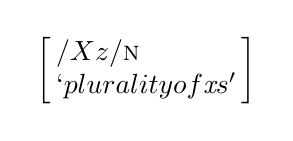
\begin{tikzpicture}
\node(RIGHT){$\left[
    \begin{array}{@{\,}l@{\,}}
        /Xz/\textsc{n}\\ 
        \text{`plurality of \textit{x}s'}
    \end{array}
    \right]$};
\end{tikzpicture}   

\ex\label{ex:wiemer:22} 
generalized\\
\begin{tikzpicture}
\node(LEFT)[]{$\left[
    \begin{array}{@{\,}l@{\,}}
        /X/\textsc{n}\\ 
        \text{`\textit{x}'}
    \end{array}
    \right]$};
\node(RIGHT)[right=of LEFT]{$\left[
    \begin{array}{@{\,}l@{\,}}
        /Xz/\textsc{n}\\ 
        \text{`plurality of \textit{x}s'}
    \end{array}
    \right]$};
\draw[<->](LEFT)--(RIGHT);
\end{tikzpicture}   
\end{exe}

What is called “words” here might better be labelled ``word forms''. While WP-approaches do not deny that words (or word forms) are often composed of smaller units, and that these units usually have meanings of their own, their endeavor is not to decompose word forms into morphemes in order to construct from them the meanings of whole word forms (in a more or less compositional manner). WP approaches do not pursue a bottom-up procedure of this kind, but, conversely, they abstract away from particular phonological realizations (and concomitant alternations in the form of purported units on a subword level) of word forms and rather analyse in a top-down manner by comparing the shape of particular word forms with their variation according to some homogeneous functional parameter(s). This principled difference – constructing larger units from smaller ones vs abstracting away from particular forms and asking for functions due to which these forms enter into replacement relations – is the reason why \citet{Blevins2016} distinguishes between ``constructive'' and ``abstractive'' models of morphology. WP approaches are clearly abstractive, while Item-and-Arrangement (IA) and Item-and-Process (IP) approaches are ``constructive'' because they rest on the basic assumption that larger units (words, phrases) are constructed from smaller ones according to certain rules.

From a ``constructivist'' viewpoint, paradigmatic relations are of no primary concern, often they are neglected or even denied altogether. In turn, ``abstractivists'' may not feel forced to assume any such units like stems (or, even more so, roots), although word schemas and correspondence rules suggest that word forms can be analyzed into smaller parts. Constructivist reasoning accepts morphemes as basic units of analysis, it has introduced allomorphs as a concept (and morphonology as an intermediate structural level) by which different phonological realizations of meaningful distinctions in word forms correlate with their phonological environment on morphological conditions. IA-models may be sufficient for purely concatenative morphology, but morphonological alternations leading to a lack of perceptual transparency already require an IP-model (\citealt[72--73]{Plungjan2000}). Up to here, no paradigmatic relationship between (the variation among) the involved units need be assumed, but no later than with suppletion a notion enters the scene which forces us to assume paradigmatic relations.

WP models have usually been called ``realizational'', since their primary interest lies in the discovery of patterns of replacement (given some sufficiently defined contextual conditions) from among a set of forms which share some lexical meaning, but also match variation with regard to certain function(s). In order to disclose such correspondences the match between word form variation and function variation must be predictable (to some minimal degree), and the more regular the pattern is in formal expression, the easier it is to discern. More traditional WP-varieties have discovered such matches on a descriptive level, while more recent WP-varieties move further by demonstrating that members of a paradigm have different weight, since some of them betray a higher degree of reliability, so that on their basis one may predict other members. That is, paradigms are often asymmetric, and parts of them are interdependent in that they provide cues for implications concerning the structure of the entire paradigm. WP-varieties which focus on these relations can be called ``implicational''. They show that paradigms supply structures which should be investigated from the point of view of information theory (and discriminative learning); cf. \citet{Blevins2016}.

Remarkably, neither the mainstream of ``constructive'' models nor the many varieties of ``abstractive'' models are very explicit about what they take to be a lexical unit, and how such units are to be identified (irrespective of form). Simultaneously, discussions about adequate models of morphology, or morphosyntax, have circled around inflection (or what is considered to be inflection), and the application of the proposed models is usually considered to be problematic for (whatever is considered) derivation.\footnote{\citet{Spencer2013} seems to be an exception. Characteristically, \citet{Spencer2020, SpencerForthc} argues for a tight mutual connection between the notions of ``paradigm'' and ``lexeme'' without “bothering” too much about an inflection-derivation divide.} The reason appears to be that derivation traditionally denies the lexical identity of the involved word forms (see \sectref{wiemer:6}). Regardless of this, apart from the attention paid (or not paid) to paradigmatic relations, a main difference between abstractivist and constructivist thinking is the format of the units that are assumed to be basic (words or, maybe, also stems vs morphemes, including roots) and the direction of analysis (``from wholes to parts'' or ``from smaller to larger units''). As for these basic assumptions, WP sides with CG.

After all, IA-, IP- and WP-models (differentiated for realizational and implicational varieties) can be ordered on a gradient (\citealt[14--17]{Blevins2016}, also \citealt{Plungjan2000}: 71--78), and probably none of them is able to lay claim to an adequate picture of linguistic reality covering all types of form-function variation in the morphosyntax of all languages. Consequently, there is per se nothing bad combining theoretical premises and analyses, provided the following alternatives are equilibrated: are grammatical oppositions (or: categorial oppositions in morphosyntax and/or on discourse level) better inferred from the combination of distinct units and rules of their combination? Or are they captured more adequately by a hierarchy of schemas and patterns for which units of lower formats are inferred via analogical proportions and replacement conditions for slots (see \sectref{wiemer:6})? This includes the question whether the “output” of combinations is transparent (=\,compositional) or not, but even more so two other things: first, one must define the format of the units that may be combined and, second, one needs to understand what triggers the grammatical (or, more broadly: categorial) opposition, i.e. which syntagmatic and/or paradigmatic cues are responsible as reliable indicators (or even predictors) of matches between oppositions in form and functional distinctions. Such considerations provide the background for the following subsection.

\subsection{Units, choices, and conditions of replacement}\label{wiemer:4.3}

To resume, the derivational patterns relevant for Slavic aspect (\sectref{wiemer:2.1}) yield stems belonging either to pfv. or to ipfv. aspect by virtue of opposite sets of functions and constraints with complementary distribution (\sectref{wiemer:2.2}). On the “morphological surface” the patterns look very heterogeneous. This is not a problem for WP- or CG-models, since they focus on schemas and correspondences. However, as was concluded in \sectref{wiemer:3}, stem derivation only provides the “input” for templates of larger constructions in which aspect assignment is not “visible” as such, since it depends on the morphological and lexical relatedness of the given stem to other stems, and it is only this relation and the membership in one of two classes (defined via opposite sets of constraints and functions) by which a binary contrast arises. This contrast is highly abstract, both in form and function. Lets therefore have a closer look at schemas and correspondence rules used in CG and WP and ask whether they can implement this contrast. See first the word-schema in \REF{ex:wiemer:21c} above and the related correspondence rule in \REF{ex:wiemer:22}, the latter replicated here for convenience:


\eabox{\label{ex:wiemer:23} 
    % \begin{figure} 
        %\includegraphics{figures/Wiemer-Bsp22.png}
\begin{tikzpicture}
\node(LEFT)[]{$\left[
    \begin{array}{@{\,}l@{\,}}
        /X/\textsc{n}\\ 
        \text{`\textit{x}'}
    \end{array}
    \right]$};
\node(RIGHT)[right=of LEFT]{$\left[
    \begin{array}{@{\,}l@{\,}}
        /Xz/\textsc{n}\\ 
        \text{`plurality of \textit{x}s'}
    \end{array}
    \right]$};
\draw[<->](LEFT)--(RIGHT);
\end{tikzpicture}    
        
    % \end{figure}
}

Here two segments are assumed: a unit bearing some lexical meaning (=\,\textit{X}), and a unit indicating a value from some grammatical category (=\,\textit{z}). The latter notion may be extended to any kind of categorial distinction (or opposition). In this example, the complex expression \textit{Xz} is classified as a form of a noun; \textit{X} may be considered a stem. Now, regardless of whether \textit{z} indicates some value of another categorial opposition as well (i.e. whether it is a portmanteau morpheme) or not, it acquires some paradigmatic value if it stands in a replacement relation with another segment (say, \textit{y}) marking, for instance, that a word form \textit{Xy} denotes a duality of \textit{X}s. Lack of either \textit{z} or \textit{y} in a word form based on \textit{X} can then be interpreted as the denotation of a single entity, provided either \textit{z} or \textit{y} otherwise always appear if a plurality or duality of \textit{X}s is referred to. This is how the standard analysis of a simple paradigm of number of nouns goes, in a simplified manner and abstracting away from possible differences in phonological realization (alias allomorphy), but implying obligatoriness.

Note that in the last example the “identifier” of the grammatical function (\textit{x}, \textit{y} or zero) belongs to a subword level. But nothing changes in principle if a correspondence rule as in \REF{ex:wiemer:22} is applied to units of other formats, for instance to words as possible parts of clause frames, e.g. German modal particles in declarative or interrogative sentences, as in the following made-up example \REF{ex:wiemer:23b}:

\ea 
\ea Ich habe schon abgewaschen.\\
    ‘I have already done the dishes.’ \label{ex:wiemer:23a}  \\

\ex \label{ex:wiemer:23b}  Ich habe \textit{ja} schon abgewaschen.\\
    ‘I have \{ja\} already done the dishes.’\\
\z\z

By using the particle \textit{ja} the speaker reminds the interlocutor(s) that the information (‘I have already done the dishes’) should be known to them. The particle thus functions as a signal that the speaker assumes the content of their message to be presupposed in the communicative space shared with the interlocutor(s). \citet{Diewald2006} and \citet{DiewaldFerraresi2008} show that this function is a general property of German modal particles\footnote{Recently, \citet{Panov2020} has demonstrated that such particles (“enimitives”) are better characterized as means to frame a proposition as uncontroversial. However, this slight shift in functional definition has no impact on the argument pursued here.}. In addition, these particles mark the utterance as non-initial in a discourse, which seems to follow by implication from the presupposition assumption. On this basis, it is easy to create a correspondence rule in which a modal particle (\textsc{\textsubscript{mp}}) contributes this kind of meaning to a very general type of construction, namely to sentences (\textsc{\textsubscript{s}}) which denote propositions (\textit{prop}) or actions (\textit{act}),\footnote{Some modal particles are also used in directives, e.g. \textit{doch}: \textit{Mach (doch)!} ${\approx}$ ‘Just do it, will you!’.} and marks them as non-initial. The form of such a correspondence rule would be analogous to \REF{ex:wiemer:22}; see \REF{ex:wiemer:23c}, ${\supset}$ means ‘implies’:

\begin{exe}
    \ex \label{ex:wiemer:23c}
    \begin{tabularx}{.95\linewidth}[t]{@{}lcQ@{}} 
    /X/\textsubscript{S} & ${\leftrightarrow}$  &  /X\textit{\textsubscript{ja}}/\textsubscript{S}, or generalized: /X\textsubscript{MP}/\textsubscript{S}\\
    ‘\textit{prop/act}’  & & ‘proposition or action presupposed and shared with interlocutor’\\
                         & & ${\supset}$ ‘non-initial in current discourse’
    \end{tabularx}
\end{exe}

Analogous correspondence rules could be created for the meaning contribution of modal auxiliaries or of any other modifiers on the level of predication, clause or sentence. Especially if their set is small, they may enter into replacement relations and, thus, form a paradigm, at least in a loose sense.

There is, of course, a difference between the “morphological” example to which the schema in \REF{ex:wiemer:22} applies, on the one hand, and modifiers on higher levels of constituency, on the other. On the morphological, i.e. word level, those parts which indicate some grammatical value (\textit{x}, \textit{y}, \textit{z} in the example above) often become obligatory in a strict sense. For instance, in German, English or Russian nouns cannot remain unspecified for number (in contrast to other languages, e.g. Turkish), even if arithmetic count proves insensible (e.g., with mass nouns). As a consequence, lack or change of some phonological segment in the word form is indicative of some value in the relevant functional domain (here: ‘1’ vs ‘>1’ or, if there is a dual, ‘1’, ‘2’, ‘>2’) or reinterpreted in accordance with whatever number marking means in non-trivial (i.e. non-arithmetic) usage contexts. In structuralist terms, this reasoning implies an equipollent contrast, while privative contrasts would not yield such effects, i.e. the functional value (trivial or non-trivial one) remains just unspecified. In ``constructivist'' approaches this reasoning leads to the postulation of zero morphemes. However, as a rule of thumb, the larger the format of constituents above word level, the worse the conditions get for postulating zero marking, and this mirrors the decrease in strictness with which one can speak of paradigmatic tightening and with which slots (within units of larger format) can be discerned. Consider modal auxiliaries (as Engl. \textit{can}, \textit{may}, \textit{must}): intraparadigmatic replacement conditions between them may become tighter, but nonetheless it is difficult to impossible to pinpoint syntactic conditions which make their use compulsory. One may possibly formulate communicative conditions under which modal auxiliaries are more likely to appear,\footnote{Compare the distinction between language-internal and communicative obligatoriness made by \citet[5]{DiewaldSmirnova2010}.} but this does not lead to the same level of predictability which can be observed with for the explicit distinction of many of the categories that are marked on words. So-called analytical inflections (e.g., periphrastic tense or mood forms) are no counterexample to this consideration, they rather confirm it, because their ``auxiliary words'' fill out positions in paradigms for functions that are expected beyond some communicative needs.\footnote{Moreover, slots filled by periphrasis usually build on already established paradigmatic relations between ``synthetic'' word forms (\citealt{Haspelmath2000}, \citealt[61--66]{Plungjan2011}, \citealt{SpencerPopova2015}).} Expectability drawn simply from communicative needs would still leave some freedom of choosing the categorial distinction as such to the speaker.

Thus, even if transparadigmatic tightening for clause- or utterance-level modifiers may occur it normally still leaves the speaker some leeway,\footnote{To continue reasoning in structuralist terms, one may say that a privative opposition (marking vs not-marking) has not yet turned into an equipollent contrast.} including the possibility to mark the categorial distinction by some other means. For instance, Diewald argues that German modal particles are compulsory for the function described above and that, consequently, the contrast between \REF{ex:wiemer:23a} and \REF{ex:wiemer:23b} implies that \REF{ex:wiemer:23a} does not convey this function (since it is, as it were, zero-marked). However, although modal particles are a very convenient, frequent and, thus, expectable way of expressing the speaker’s presupposition in German, it seems too categorical to deny utterances without modal particles the possibility to induce such presuppositions, e.g. just by intonation, i.e. to deny that utterances without modal particles can be used if the speaker wants to express such a presupposition.\footnote{Modal particles are a bad example also for the reason that, at least in German, they can be combined in the same utterance; they are thus not even organized in stricter paradigmatic replacement conditions.}

After all, regardless of how this issue may be further settled, “morphological examples” like number marking on nouns and modifiers of higher levels of constituency have one thing in common despite all other differences: they can be spelt out by pointing to distinct elements (traditionally called morphemes, words, etc.) or at least to constructions (with different complexity of constituency). This sets them apart from obligatoriness conditioned by the choice of verb stems, which in Slavic languages is inevitably connected to aspect; this choice is binary and, apart from a limited amount of biaspectual (or anaspectual) stems, one cannot circumvent it. The latter property, namely: lack of transparadigmatic variability, is similar to number on nouns (in Slavic, Germanic, and Romance languages), but different from what can be found with, for instance, modal auxiliaries and arguably with modal particles as well. Concomitantly, it is not bound morphology as such that triggers the distinction between aspect, but derivational patterns (i.e. the relation between two or more stems) correlated with sets of functions and restrictions.

Moreover, the affixes which relate verb stems to each other attach prior to any tense or person/number marking (or suffixes deriving non-finite forms). That is, although the patterns work on a subword level, it is not the simple concatenation of morphemes that is crucial but the relation between stems, which is intermediary between word and morpheme. In addition, one has to account, first, for the degree of lexical closeness between the involved stems and, second, often also for the step at which the respective affixes attach in a derivational chain (see \sectref{wiemer:2.1}). That is, what is implied by these patterns cannot be captured simply as constructions or by correspondence rules of the type illustrated above. Rather, templates are needed which, to a certain extent, include rule-based information about, first, the procedure of how to “get” one stem from another and, second, about alternations in phonological form (which are frequent and predictable, for instance, at the border between stem and imperfectivizing suffix). However, regardless of whether one allows for rules (operating on stems, not on words) or relies only on schemas, it has to be admitted that, in analogy to \REF{ex:wiemer:22}, what corresponds to \textit{Xz} cannot be subdivided into a part which specifies the aspect value (pfv. vs ipfv.) and a part which bears the lexical meaning.\footnote{Or, in analogy to \REF{ex:wiemer:23c}, into a part denoting propositional content and its modifier.} That is, neither an abstractive (WP, CG) nor a constructive (IA or IP) approach brings us to the ultimate goal; one seems better advised to combine elements of both (see \sectref{wiemer:4.2}). What the \textit{Xz} corresponds to is most often only infinitive or present/non-past tense stems (“allostems”), e.g. Russ. \textit{pisa}{}- or \textit{piš}{}- ‘write.\textsc{ipfv}’ or Pol. \textit{przepis-ywa}{}- or \textit{przepis-uj}{}- ‘write anew.\textsc{ipfv}’. The same applies if something precedes \textit{X}, i.e. a prefix, as in \textit{na-pisa}{}- vs \textit{na-piš}{}-.\textsc{pfv} (see \ref{ex:wiemer:3}--\ref{ex:wiemer:4}). Moreover, even if the notion of allomorphy is acknowledged in one’s analysis, it is appropriate for morphonological changes that distinguish the present (or non-past) from the infinitive stem, but entirely inappropriate for variability in the choice from 15+ verbal prefixes, which in most cases change lexical meaning, but also may serve to simply indicate that the unit is a pfv. verb (see \sectref{wiemer:2.1}). That is, a correspondence rule like /X/ (‘\textit{x}’) ${\leftrightarrow}$ /\textsc{\textsubscript{pfx}}X/ (‘pfv. of \textit{x}’) would apply only to a limited number of aspect pairs and triplets; it does not reflect the dual character of verbal prefixes as changes of (partial) word-forms that indicate pfv. aspect, but in most cases also modify the lexical meaning (which jeopardizes the relation between \textit{X} and \textsc{\textsubscript{pfx}}\textit{X} out of a paradigm of forms which realize the same lexical unit). Nor does it help to understand in which cases, nonetheless, \textsc{\textsubscript{pfx}}\textit{X} just means ‘pfv. of \textit{x}’ (as with Natural Perfectives), among a couple of other issues.

Nothing changes for all these considerations if, instead, a more complex correspondence rule is applied, e.g. a schema as in \REF{ex:wiemer:20}. That the applicability of correspondence rules (or schemas) may depend on the format of the units which, in some way or another, have to be assumed on a subword level. They cannot simply be transferred from a morpheme level to stems in particular if the change of the stem itself carries information about the value of the grammatical opposition (pfv. vs ipfv.), i.e. subtractive of tense and agreement or non-finiteness markers, which are only added to these stems.\footnote{Even from a constructivist perspective, one would not say that an unprefixed ipfv. stem has a “zero prefix” by which imperfectivity is marked, or conversely that prefixed pfv. stems have a “zero suffix” since their ipfv. counterparts are often marked by an extra suffix (at least, I am ignorant of any such attempt).} In addition, the aspect value hinges on patterns of stem changes that are not unified: not only are there two predominant patterns with different directions of derivation (see \figref{fig:wiemer:predom}), but many idiosyncratic ones (mostly obsolete remnants of earlier layers of stem derivation); there is even one pattern which is based on a monofunctional suffix creating pfv. stems, but only in the confines of a specific semantic class of atelic stems (or lexemes, for that matter), namely semelfactive \{nǫ\} (see \sectref{wiemer:2.1} and \sectref{wiemer:3}).

Even from a strict ``constructivist'' point of view it would be totally off the mark to try to subsume such a variation of patterns on the “morphological surface” under allomorphy (and presumably nobody has tried to do so). For ``abstractivists'' the problem differs, namely: can a common paradigm for some pfv. and ipfv. stem be imagined, provided there is reason to assume that they share an identical lexical concept or are even close synonyms? This problem cannot be tackled with correspondence rules. Therefore, it seems reasonable to consider whether paradigms may be based not so much on the form of particular stems (and of how they are composed from morphemes) and not too much tied to specific patterns of stem derivation, but, instead, primarily built on categorial restrictions on different levels of morphosyntax and discourse which yield a sufficiently reliable distribution, or patterns, of oppositions tied to the choice between pfv. and ipfv. stems. These patterns may be described with templates, but in a form which at present hardly anybody would want to call ``constructions''.

How can these insights be exploited for modeling the architecture of Slavic aspect? And, conversely, what can be gained for morphological theory, or a theory of grammatical categories? The last two sections explore these questions.

\section{Extended notion of paradigms: A proposal}\label{wiemer:5}

The proposal rests on two pillars. First, aspect choice is obligatory, and since this choice amounts to making a decision between verb stems it is these stems which are in paradigmatic opposition for an abstract feature, namely PFV:IPFV. Then, second, the question is what determines this choice in the first place. As explained above (mainly in \sectref{wiemer:2.2}), verb stems are ascribed pfv. or ipfv. aspect according to sets of functions and grammatical constraints over which they distribute in a (more or less) complementary manner. By virtue of these sets verb stems belong into one of two opposite classes, so that a binary opposition is established. These conditions justify considering Slavic aspect as a classificatory category. By the same token, issues like how many aspect pairs (or triplets) there are, and how regular the morphological relations between lexically close stems are, are important only to the extent that there must be some backbone of the system in order to (i) supply regular patterns of derivation to be applied productively, and in order to (ii) establish paradigmatic replacement conditions between stems denoting identical (or very close) lexical concepts, i.e. to create minimal pair conditions (as exemplified throughout this paper). This backbone in terms of formal patterns and of lexical relatedness provides the basis for analogical transfer, both for the productive application of rules (or schemas) and for relating stems of opposite aspect with obsolete or less frequent patterns, briefly: for the integration of new and old stems into a system which distributes them over two classes defined via sets of constraints and functions.

Consequently, there is a maximally simple paradigm to start with, which is conditioned by an inevitable binary choice: either a member of the ipfv. class or a member of the pfv. class, whatever other grammatical categories might be expressed by a verb, and in whatever discourse context. Whenever a verb is involved in a categorial (grammatical or pragmatic) contrast, this influences aspect choice – since speakers cannot avoid it. The associations between aspect choice and the value of the contrast are reliable (and predictable) to different degrees, so core and peripheral (or stronger and weaker) conditions (or factors) may be distinguished. Concomitantly, there is no general rule saying that a particular morpheme indicates pfv. or ipfv. aspect as such. Thus, the aspect value is a factor that should be accounted for not only as a distinct element of constructions, but as something that can be visualized with templates, which I take to be sets of properties ordered by levels, or components. This distinguishes templates from constructions, or schemas, which are primarily characterized by their syntagmatic “outfit” and which normally lack a complex structure of levels (see the representation in \REF{ex:wiemer:20} and the correspondence rules above). By contrast, the templates require up to five components:

\begin{enumerate}[label=(\roman*)]
    \item aspect (pfv. vs ipfv. stem),
    \item grammatical form of the stem (i.e. whatever may be added on the stem: markers of tense and agreement, or non-finiteness),
    \item other markers (e.g., negation, auxiliaries, temporal adverbials),
    \item actionality and reference (i.e. functions constituting the core of any aspect opposition, incl. event-external pluractionality and temporal definiteness a.k.a. episodicity),
    \item pragmatic function (e.g., illocutionary purpose, presupposition management).
\end{enumerate}

Components (i) and (ii) are indispensable, since they are always specified morphologically (as any verb form in Slavic). Components (iv) and (v) are also indispensable, but only in the sense that these properties are inherent to any utterance, even without explicit specification. Elements of component (iii), in turn, are optional. Simultaneously, (ii) and (iii) represent distinct linguistic material (as units on a word and subword level) which interfere with aspect (as inherent to the stem) on a syntagmatic axis; (ii) and (iii) can specify parts of larger constructions (on predication or clause level) accessible for a description in CG terms or for correspondence rules in a WP fashion. The other components are non-distinct and, in this respect, abstract. After all, each of the components itself implies paradigmatic contrasts (between forms or functions), but the assignment of aspect, i.e. (i), provides the basic binary paradigmatic distinction.\footnote{For this reason no additional level has to be assumed (contrary to what one of the reviewers suggested): by the choice of ipfv. or pfv. aspect the opposition to the other aspect (= grammatical class) is determined ipso facto (\textit{tertium non datur}). See also the peg-metaphor below.} In this sense, aspect choice is like a pivot, since in combination with the other components it participates in the formation of minimal pair contexts (part of which was illustrated in \sectref{wiemer:2}).

A template can be created for each categorial distinction for which aspect choice is a sufficiently reliable indicator, or by which it is restricted; the other factors which also contribute to this distinction (or condition the restriction) are listed as components (ii-v). The “nature” of the categorial distinction is used as a label of the template (maybe together with the language or subdivision of Slavic to which it applies); it is, as it were, the minimal common denominator for the contrast conditioning aspect choice. The symbol ``---'' means that no specification is required, properties in parentheses are optional, additional information is given in brackets.

An illustration of a relatively simple template would be the formation of the future tense of ipfv. and pfv. stems in North Slavic; see \tabref{tab:wiemer:xx}.

\begin{table}
\caption{Future in North Slavic\label{tab:wiemer:xx}}
\begin{tabularx}{\textwidth}{l@{ }ll@{ }Q}
\lsptoprule
(i)   & IPFV                                        & (i)   & PFV\\
(ii)  & infinitive [or \textit{l}{}-form in Polish] & (ii)  & non-past stem\,+\,non-past endings\\
(iii) & \textsc{bǫd}{}- [auxiliary]                 & (iii) & {}--- [auxiliaries excluded]\\
(iv)  & {}---                                       & (iv)  &  {}---\\
(v)   & {}---                                       & (v)   & {}---\\
\lspbottomrule                                      
\end{tabularx}
\end{table}


Here, aspect choice bears on the choice of grammatical forms and their interpretation, regardless of which functions might be associated to pfv. and ipfv. future; that is why (iv) and (v) are left unspecified.

For South Slavic the situation changes insofar as non-past pfv. stems do not yield a default future reading. Instead, a distinct future marker (Bulg. \textit{šte}, Mac. \textit{{\'к}e}, inflected Srb.-Cr. \textit{ću} and Sln. \textit{bom}) combines with either aspect and the non-past of pfv. stems is tightly associated with irrealis functions (first of all habitual, modal, conditional); it must be combined with distinct irrealis markers, among which for most of these languages \textit{da} is the predominant one.\footnote{Alternatively, one might say that future belongs to the irrealis domain and that, correspondingly, the future morpheme itself marks irrealis. The consequence would be that South Slavic does not have future marking, or that future is but a standard (or generalized) implicature of non-past + the respective irrealis marker. This, however, would not change anything essential in the template (see \tabref{tab:wiemer:xy}).} Thus, for South Slavic non-past pfv. stems the template is as in \tabref{tab:wiemer:xy}.

\begin{table}
\caption{Non-Past in South Slavic\label{tab:wiemer:xy}}
\begin{tabularx}{\textwidth}{l@{ }ll@{ }Q}
\lsptoprule
(i)   & IPFV                             & (i)  & PFV\\
(ii)  & non-past stem\,+\,non-past endings & (ii) & non-past stem\,+\,non-past endings\\
(iii) & \textsc{{}---}                   & (iii)&  \textsc{irrealis} [e.g., \textit{da}]\\
(iv)  & {}---                            & (iv) & suspension of assertivity [‘non-actual present’]\\
(v)   & {}---                            & (v) & {}---\\
\lspbottomrule
\end{tabularx}
\end{table}

Another minimal pair contrast, widespread all over Slavic, is aspect in the imperative +/$-$ negation. See (\ref{ex:wiemer:10a}--\ref{ex:wiemer:10b}), adduced in \sectref{wiemer:2.2} and replicated here as \REF{ex:wiemer:24}, and the corresponding template in \tabref{tab:wiemer:yz}.

\ea \label{ex:wiemer:24}
{Russian} \\ \ea 
    \textit{Ne rasskaži}\textsc{\textsuperscript{pfv}} emu (slučajno), čto ty videl.\\
    ‘\textit{Don’t tell} him (inadvertently), what you have seen.’ \label{ex:wiemer:24a} \\
    \ex \label{ex:wiemer:24b} Nu, čto ty tam videl? (Ty obeščal mne rasskazat’\textsc{\textsuperscript{pfv}}.) \textit{Rasskazyvaj}!\textsc{\textsuperscript{ipfv}}\\
    ‘Well, what have you seen there? (You promised to tell me.) \textit{Tell} me.’
\z \z 

\begin{table}
\caption{Directive speech acts}
\label{tab:wiemer:yz}
\begin{tabularx}{\textwidth}{l@{ }Ql@{ }Q}
\lsptoprule
(i)   & IPFV &              (i)   & PFV\\
(ii)  & imperative &        (ii)  & imperative\\
(iii) & negation &          (iii) & no negation\\
(iv)  & (single instance) & (iv)  & single instance\\
(v)   & directive and deontic: prohibition [addressee is assumed to have control over event denoted by the verb] & (v) & directive and deontic: order, command, request, etc. [addressee is assumed to have control over event denoted by the verb]\\
\lspbottomrule
\end{tabularx}
\end{table}

For the ipfv. imperative (with negation) the referential condition is given in brackets because prohibitives do not imply the exertion of social force for single occasions; they can be (and often are) uttered as a general command (e.g., \textit{Don’t eat with your fingers}). However, provided the directive speech act refers to a single situation (with a concrete illocutionary concern), pfv. and ipfv. stems are in an ideal paradigmatic replacement condition, and this applies to virtually all Slavic languages: the illocutionary background (a deontically, i.e. socially motivated directive speech act) does not change, only negation makes the difference and “switches” the aspect. 

A complication arises inasmuch as the negated ipfv. imperative is used for other purposes as well (see \sectref{wiemer:2.2}). A similar point holds for unnegated ipfv. imperatives which, among other grammatical forms of unnegated ipfv. stems, are employed to signal that the speaker assumes the relevant action to be presupposed (also by the interlocutor). Other grammatical contexts without negation in which ipfv. stems are associated with this discourse function are modals (compare ex. \ref{ex:wiemer:12a}--\ref{ex:wiemer:12b}) or the future tense. Slavic languages obviously differ as for the prominence of this function, but it anyway often interferes with other functions associated with ipfv. aspect. An analogous point concerns event-external pluractionality, in particular the denotation of unrestricted repetition, which systematically conflicts with actional defaults and the limiting function of the pfv. aspect.\footnote{This conditions an inner-Slavic differentiation of the factor hierarchy relevant for aspect choice (cf. \citealt{Dickey2000}: Ch. 2, \citealt{Wiemer2008}: 399--403, among others).}

Furthermore, as templates like \tabref{tab:wiemer:xy} show, one of the two aspects may not require any further specification, i.e. its use is rather unrestricted, while the other aspect is subject to quite severe restrictions. Such an asymmetry also holds true for more complex cases, as with negated imperatives in which the employment of pfv. stems requires very specific conditions (which, in addition, may be more salient only for a particular subarea of Slavic) that are not visible just “on the surface” (see \citealt{WiemerForthcoming}). In other clear cases of asymmetry one of the aspects is altogether blocked, not because of some specific (and shaky) context conditions, but for a more straightforward reason. This is the case with aspect in the scope of phasal verbs\footnote{Note that phasal verbs themselves distinguish aspect, i.e. most of them come in pairs, so that their own aspect is indicative of the same functions and constraints as for other verbs.} which, as mentioned in \sectref{wiemer:2.2}, allow only for ipfv. stems in any Slavic language (except colloquial Upper Sorbian). The template looks, therefore, like \tabref{tab:wiemer:zy}; * symbolizes blocking.

\begin{table}
\caption{Aspect in the scope of phasal verbs}
\label{tab:wiemer:zy}
\begin{tabularx}{\textwidth}{l@{ }Ql@{ }Q}
\lsptoprule
(i)   & IPFV &  (i) & *PFV\\
(ii)  & infinitive [North Slavic and Slovene]\slash\textit{da} + non-past stem + non-past endings [South Slavic] & (ii) & infinitive [North Slavic and Slovene]\slash \textit{da} + non-past stem + non-past endings [South Slavic]\\
(iii) & \textsc{phasal verb} & (iii) & \textsc{phasal verb}\\
(iv)  & {}--- & (iv) & {}---\\
(v)   & {}--- & (v) & {}---\\
\lspbottomrule
\end{tabularx}
\end{table}

Of course, the blocking of pfv. aspect by phasal verbs is motivated, as the general meaning of pfv. aspect consists in setting limits, and this meaning conflicts with the semantics of phasal verbs. In fact, there is reason to argue that most (if not all) of the functional contrasts and constraints on aspect choice are motivated from the basic categorial distinction between setting (or foregrounding) limits of situations (${\rightarrow}$ PFV) and backgrounding them (${\rightarrow}$ IPFV), and only part of the contrasts and constraints can additionally be motivated by telicity.\footnote{In other words, telicity provides a condition for subsets of the inventories of functions and constraints associated to ipfv. vs pfv. aspect.}

There is no place (or need) to continue with illustrations of what templates might look like if one wants to capture not only the formal properties of constructions and involved verb forms, but also their functional interpretation for different types of utterances. Hopefully, the general idea has become clear. The crucial point is that every template is based on a choice between pfv. and ipfv. stem; this choice cannot be avoided once verbs are involved, and all properties from (ii) to (v) are “linked” to a pfv. or ipfv. stem (= (i)) like pieces of clothing hanging on pegs, either as unequivocal decisions or as salient tendencies. These pegs (= ipfv. vs pfv. stems) provide the basic paradigmatic contrast, regardless of whether the function (or constraint) concerns (plur)actionality features or bears relevance to temporal deixis (as with the default present > future shift for pfv. stems in North Slavic), or the functional contrast is at best remotely related to these core domains of aspect oppositions.

Conflicts between these factors are unavoidable since the pfv.:ipfv. opposition supplies only a binary choice, and since sense has to be made out of this choice even if actionality or pluractionality features are irrelevant or remain in the background. However, analogous conflicts arise with other binary oppositions and obligatory choices (i.e. if transparadigmatic variability is minimized or lost), such as singular-plural distinctions for nouns in most European languages or a definite article, e.g. in Balkan Slavic. The difference, again, is that these categories (and the corresponding paradigmatic contrasts) are not marked by stems (as is Slavic aspect).\largerpage[1.5]

The templates are able to integrate correspondence rules (or schemas), if aspect choice reliably hinges on some syntagmatic condition, for instance on some contextual element like \textit{bud}{}- for the ipfv. future in Russian or Czech, or on an irrealis marker (like \textit{da}) for pfv. present in Balkan Slavic. However, since simple constructional approaches are unable to capture the classificatory properties of Slavic aspect arising from sets of functions and constraints, and since this opposition is morphologically based on different derivational patterns, only templates can do the job of relating the paradigmatic opposition of pfv. vs ipfv. stems to the functional contrasts and grammatical constraints which have been discussed in the literature on Slavic aspect and in a flashlight manner throughout this article.

This said, a further step can be taken by reinterpreting \emph{sets} of such templates as members of paradigms of aspect choice. That is, \emph{each template}, regardless of how complex its internal structure, \emph{equals a paradigm cell}, but elements of its internal structure are linked to other layers of the overall paradigm. The entire paradigm would then consist of two layers (see \figref{fig:wiemer:5}).\footnote{This proposal remotely resembles Leino's “metaconstructions” \parencitetv{chapters/03_leino}, as far as analogy is at play. However, whereas metaconstructions are conceived of as generalizations of constructions, two-layer paradigms as developed here are much more characterized by internal relations between particular components which depend on the binary choice between pfv. and ipfv. stems.} Stems (each with its aspect) distinguish gamuts of finite and non-finite forms which make up paradigms in the traditional sense, and these constitute the first layer. Whether one wants to deal only with the set of finite forms, or whether one includes also non-finite forms (and which ones) into the paradigm, is of secondary concern. The smaller set of finite forms may be called ``narrow'' or ``classical paradigm'', the larger set which includes non-finite forms ``extended paradigm'', and the latter is still needed. The issue of periphrastic forms which fill out cells of traditional paradigms (“analytical inflection”), such as, e.g., the future of ipfv. verbs in North Slavic (person-number inflected auxiliary \textit{bud}{}- plus infinitive of ipfv. stem), is of secondary concern, too. The reasons were discussed in \sectref{wiemer:4.3}.

The templates of the type illustrated above provide the second, more abstract layer. Component (i) of each template is the paradigmatic opposition between ipfv. and pfv. stem itself, i.e. the pegs on which everything hinges. As inherent to stems, it ties together all templates from the same column (= vertical axis). Component (ii) cross-references forms from the extended paradigm (= first layer), it thereby specifies which of these forms are relevant for the given template and, together with component (i), supplies a connection between first and second layer.\footnote{How this might be done technically should be considered separately.} The basic structure of such a complex, two-layer paradigm is shown in \figref{fig:wiemer:5}. As shown above, the relation between the pfv. and ipfv. halves of the templates may be asymmetric, either in form-related conditions or in the functional conditions applying to one of the stems in the paradigmatic relation.\largerpage[1]

\begin{figure}\small
\begin{tikzpicture}[row 3 column 3/.style={anchor=base}]
  \matrix (matrix) [matrix of nodes, nodes in empty cells, nodes={anchor=base west}]
    {traditional paradigm &[1em] IPFV stem &[1em] PFV stem\\[.25cm]
     narrow paradigm & finite forms & finite forms\\[1.25cm]
     extended paradigm & +non-finite forms & +non-finite forms\\[1.25cm]
                       & IPFV & PFV\\
                       & component (i) ipfv & component (i) pfv\\
       template 1      & component (ii)  & component (ii)\\
                       & component (iii--v)  & component (iii--v)\\[1cm]
                       & component (i) ipfv & component (i) pfv\\
       template 2      & component (ii)  & component (ii)\\
                       & component (iii--v)  & component (iii--v)\\[1cm]
%                        & component (i) ipfv & component (i) pfv\\
%           $\vdots$     & component (ii) ipfv & component (ii) pfv\\
%                        & component (iii--v) ipfv & component (iii--v) pfv\\[1cm]
                       & component (i) ipfv & component (i) pfv\\
         $\vdots$      & component (ii)  & component (ii)\\
                       & component (iii--v)  & component (iii--v)\\[1cm]
                       & component (i) ipfv & component (i) pfv\\
        template $n$   & component (ii)  & component (ii) \\
                       & component (iii--v)  & component (iii--v) \\                       
    };
    \node (subset) [fit=(matrix-2-2), draw, dashed, inner sep=0pt] {};
    \node [fit=(matrix-2-3), draw, dashed, inner sep=0pt] {};
    
    \node (superset) [fit=(matrix-3-2) (matrix-2-2), draw, inner sep=3pt] {};
    \node (superset2) [fit=(matrix-3-3) (matrix-2-3), draw, inner sep=3pt] {};
    
    \draw [bend right, dashed] (matrix-2-1) to (subset);
    \draw (superset.212) -- ++(-1.25em,0);
    
    \draw [dashed, ->, in=180, out=220] (superset) to (matrix-6-2.west);
    \draw [dashed, ->, in=0, out=315] (superset2.south east) to (matrix-6-3.east);

    \coordinate[right=1.5em of matrix.35] (anchor-3);
    \coordinate[right=1.5em of matrix.north east] (anchor-1);
    \coordinate[right=1.5em of matrix.south east] (anchor-2);
    \draw [decorate,decoration={brace, amplitude=10pt,raise=4pt}] (anchor-1) -- (anchor-3) node [midway,sloped,above=1.25em] {First layer};
    \draw [decorate,decoration={brace, amplitude=10pt,raise=4pt}] (anchor-3) -- (anchor-2) node [midway,sloped,above=1.25em] {Second layer};
% 
% 
% 
% \node(a0)[text width=3.2cm]{IPFV};
% \node(a1)[below=5mm of a0,text width=3.2cm]{\BWcelli};
% \node(a2)[below=5mm of a1,text width=3.2cm]{\BWcelli};
% \node(a3)[below=5mm of a2,text width=3.2cm]{\BWcelli};
% \node(a4)[below=5mm of a3,text width=3.2cm]{\BWcelli};
% \node(a5)[below=5mm of a4,text width=3.2cm]{\BWcelli};
% \node(a6)[below=5mm of a5,text width=3.2cm]{\BWcelli};
% 
% 
% \node(b0)[right=5mm of a0,text width=3.2cm]{PFV};
% \node(b1)[right=5mm of a1,text width=3.2cm]{\BWcellp};
% \node(b2)[right=5mm of a2,text width=3.2cm]{\BWcellp};
% \node(b3)[right=5mm of a3,text width=3.2cm]{\BWcellp};
% \node(b4)[right=5mm of a4,text width=3.2cm]{\BWcellp};
% \node(b5)[right=5mm of a5,text width=3.2cm]{\BWcellp};
% \node(b6)[right=5mm of a6,text width=3.2cm]{\BWcellp};
% 
% \node(t1)[left=5mm of a1, text width=2cm]{template 1};
% \node(t2)[left=5mm of a2,text width=2cm]{template 2};
% \node(t3)[left=5mm of a3,text width=2cm]{\ldots};
% \node(t4)[left=5mm of a4,text width=2cm]{template i};
% \node(t5)[left=5mm of a5,text width=2cm]{\ldots};
% \node(t6)[left=5mm of a6,text width=2cm]{template n};
% 
% \node(a-1)[above=of a0]{+non-finite forms};
% \node(b-1)[above=of b0]{+non-finite forms};
% 
% \node(a-2)[above=of a-1,ellipse,draw]{finite forms};
% \node(b-2)[above=of b-1,ellipse,draw]{finite forms};
% 
% \node(a-3)[above=of a-2]{IPFV stem};
% \node(b-3)[above=of b-2]{PFV stem};
% 
% 
% \node(t-3)[left=of a-3]{traditional paradigm};
% \node(t-2)[left=of a-2]{narrow paradigm};
% \path let 
% \node(t-1)[left=of a-1]{extended paradigm};
% 
% \node(x-3)[right=of b-3]{\textsc{first layer}};
% \node(x3)[right=0mm of b3]{\textsc{second layer}};
% 
% \node(box1)[fit=(a-1)(a-2),draw]{};
% \node(box2)[fit=(b-1)(b-2),draw]{};
% 
% \draw[dashed](t-2)--(a-2);
% \draw[](t-1)--(box1);
% \draw[dashed,->](box1)--(a1);
% \draw[dashed,->](box2)--(b1);
\end{tikzpicture}
\caption{Complex, two-layered paradigms of Slavic verb stems. Broken line/arrow = cross-references with element(s) in a component (ii) of templates\label{fig:wiemer:5}}
\end{figure}

Each column in toto is opposed to the respective other column, just as, for instance, in a traditional paradigm of inflected nouns singular and plural are opposed for the category number “across” morphological cases and for stems of different gender. Admittedly, this analogy is not perfect since a traditional paradigm of inflected nouns (or verbs) has a closed set of cells, while the number of templates specifying the conditions of aspect choice can be less easily limited; it increases with every grammatically or pragmatically definable contrast for which aspect choice proves relevant. However, the amount of templates hardly constitutes an open class, either, since these contexts cannot increase \textit{ad libitum}; otherwise aspect choice would not be salient and reliable enough. Apart from this, there are other paradigms in “hard core” grammar whose closedness is debatable; consider, for instance, voice-related distinctions, paradigmatic relations between preverbs (e.g., in Germanic or Latvian), or German modal particles (see \sectref{wiemer:4.3}).

Another objection might be that the templates are not mutually exclusive, as many of them are either interrelated (by common motivation), or they can conflict with one another (see examples above). This makes the inventories of opposed templates dissimilar to cells in traditional paradigms. However, recent work in WP-morphology on traditional paradigms has shown that paradigms are often asymmetric in that their members betray an unequal status, in particular. Because some of them are better predictors for others but not vice versa. In general, paradigm members are better characterized as a network (see \sectref{wiemer:6}). Such network relations can as well be found in the sets of templates and the complex two-layer paradigms of \figref{fig:wiemer:5}. Therefore, the architecture of traditional paradigms and the principles organizing complex two-layer paradigms do not seem that different. After all, it is an unavoidable binary choice between pfv. and ipfv. aspect which makes this network arise and stabilize.

Now, if such complex, two-layered paradigms can be acknowledged, what follows from this for (morphologically related) stems of opposite aspect which are so closely related in their lexical meaning that they can be considered synonyms? This question arises regardless whether one speaks about pairs, triplets or larger groups of stems. Why not assume that stems united in this way under one lexical meaning actually share into one (though more complex) paradigm? And if the answer is positive, does this entail that these stems are to be considered representatives of the same lexical unit (= lexeme)? The last question arises because synonyms are usually treated as distinct lexemes, however, the synonyms under consideration here are morphologically related and show complementary distribution over grammatically and/or pragmatically defined contexts.\largerpage

As pointed out in \sectref{wiemer:3}, the assumed 1:1-relation between lexeme and paradigm has forced many to interpret the different stems as inflection, with diverse artificial and ad hoc “solutions”. Alternatively, if treated as a classificatory system, each stem can be ascribed its own paradigm, but this alternative is based on the same 1:1-assumption between lexeme and paradigm. Notably, nothing changes with suppletion, since suppletion itself presupposes tight paradigmatic relations and extreme closeness of lexical relatedness. Actually, suppletive aspect pairs force us to acknowledge that the grammatical value (pfv. vs ipfv.) is a property of the stem\footnote{As a reviewer remarked, since both WP and CG treat word forms as wholes, they can deal with suppletion, syncretic and analytic forms in the same way. While this is correct, it should be remembered that both syncretic and analytic forms, as well as suppletive aspect pairs, presuppose stems. Thus, as far as aspect in Slavic is concerned, stems are more basic than anything else.} (cf. \citealt[149--150]{Wiemer2020b}). Therefore, as concerns stems that are morphologically related and can be considered lexical synonyms, but show complementary grammatical behavior, I do not see any inherent reason why one should not admit for complex, two-layered paradigms composed of the extended traditional paradigms and sets of templates assigned to two related stems. These stems can each be considered separate lexemes which complement each other. Thus, instead of either of the representations given in \figref{fig:wiemer:4} (see \sectref{wiemer:3}), consider the one in \figref{fig:wiemer:4b}.

  
\begin{figure}
%\includegraphics[width=\textwidth]{figures/Wiemer-fig4b.png}
 \caption{Alternative view on the grammatical status of aspect pairs\label{fig:wiemer:4b}}
\begin{tikzpicture}
\node(inventory)[rectangle,draw, text width=5cm]{set of combinatorial restrictions};
\node(set)[rectangle,draw, text width=5cm, , left=of inventory ]{inventory of word forms\\ (finite, non-finite)};
\node(function)[rectangle,draw, text width=5cm, below=5mm of inventory, xshift=-3cm]{function inventory};
\node (bottombox) [rectangle,draw, fit=(inventory)(set)(function)] {};
\node (ONE) [rectangle, draw, text width=5cm, above=of set] {``Paradigmaticist'' viewpoint\\PFV--IPFV pair\\\textit{Two} (synonymous) lexemes\\~};
\node (TWO) [rectangle, draw, text width=5cm, right=of ONE]  {\textit{One} (complex) paradigm};

\draw[->, line width = 0.5mm](ONE)--(TWO);
\draw[->](TWO)--(bottombox.north);
\end{tikzpicture}
\end{figure}


As for aspect triplets (of either kind discussed in \sectref{wiemer:2.1}), the only thing to be admitted further is to include a third stem. For the competing pfv. or ipfv. stems one may observe different biases for subsets within combinatorial restrictions and/or the function inventory, i.e. for properties specified in templates.\footnote{\textrm{Compare, for instance, the usage-based case study in \citet{WiemerEtAlForthc}, which shows that Pol.} \textrm{\textit{dzielić}}\textrm{\textsc{\textsuperscript{ipfv1}}} \textrm{and} \textrm{\textit{rozdzielać}}\textrm{\textsc{\textsuperscript{ipfv2}}} \textrm{(pfv.} \textrm{\textit{rozdzielić}}\textrm{) and their Czech cognates} \textrm{\textit{dělit}}\textrm{\textsc{\textsuperscript{ipfv1}}} \textrm{and} \textrm{\textit{rozdělovat}}\textrm{\textsc{\textsuperscript{ipfv2}}} \textrm{(pfv.} \textrm{\textit{rozdělit}}\textrm{) ‘divide, separate’ have different preferences for stative (IPFV1) vs habitual (IPFV2) contexts.}} The same reasoning can be extended to actionality groups consisting of stems of either aspect, as argued for by \citet{Tatevosov2016}; see \sectref{wiemer:3}.

The assumptions underlying \figref{fig:wiemer:4b} also do justice to the classificatory character of the PFV:IPFV opposition. Simply those verbs for which no morphologically related stem with a close enough lexical meaning exists (\textit{perfectiva} and \textit{imperfectiva tantum}), certain parts of the paradigm, defined via word forms (= traditional paradigms), constraints and functions are absent. This can be compared to analogous cases, for instance to \textit{pluralia} and \textit{singularia} \textit{tantum} (or nouns with a strong bias to either singular or plural in non-arithmetic contexts) in relation to the values of number in nouns, or with the paradigms of verbs that do not passivize in a language with an otherwise fully developed distinction between active and passive voice. Like inventories of word forms, function inventories and sets of combinatorial restrictions (i.e. the “ingredients” of templates) are defined for a maximum range of pfv. and ipfv. stems, but they do not (and cannot) apply to every single representative of these classes; rather they are like repositories supplying admissible functions for these representatives.

One final question, alluded to above, remains. The templates which constitute the second layer of the complex paradigms can be listed; but is there some internal order between them? In particular, can some templates be regarded as more important inasmuch as they serve as predictors for other templates? Similar key functions of members in paradigms have attracted attention particularly in most recent implicational varieties of WP (see \sectref{wiemer:4.2}). It would be instructive to learn whether there exist implicational relations between templates relevant for aspect choice that parallel (or are analogous to) such asymmetries in traditional paradigms, or between constructions that are organized more tightly in paradigmatic terms.\footnote{I am unaware of any attempt in CG to disclose implicational hierarchies, or asymmetries, among constructions (apart from standard assumptions about inheritance relations; see \sectref{wiemer:4.1}).}

In fact, some templates relevant for aspect choice are certainly more important, either because the functions and/or constraints which they capture are more frequently encountered and less restricted by lexical meaning (e.g., most pluractional meanings are rather insensitive to actionality properties, including telicity), or because they are more firmly associated with their context conditions (e.g., with communicative intentions) or more difficult to suppress by conflicting conditions than constraints and/or functions specified by other templates. These constraints and functions would play a more central role in the grammar. However, relations between them are often hard to pin down, let alone to quantify. Of course, we may start with certain “hard core” constraints like, for instance, the compulsory use of ipfv. stems instead of pfv. counterparts in the narrative present tense in East Slavic and Polish, in contrast to, e.g., Czech or Slovene (see \sectref{wiemer:2.2}). But then the problem is whether such factors of aspect choice correlate with others like, for instance, the restriction of the ``inchoative'' future (with \textsc{bǫd-}) to ipfv. stems (typical of all North Slavic languages), or functional contrasts of aspect choice in the scope of modals (which show an overlay of different contrasts that can easily conflict with each other). Finally, even if sufficiently robust correlations can be disclosed, the question arises in which direction the implication goes (or whether it is bidirectional).

These questions are intriguing also for the reason that implicational relations between members of traditional paradigms seem to be arbitrary in the sense that no semantic motivation can be found; they usually just serve as an internal principle of the organization of paradigms,\footnote{Cf. \citet[172--174]{HaspelmathSims2010} on Priscianic formations.} possibly conditioned by the reduction of conditional entropy (\citealt{MilinEtAl2009}, \citealt[7]{Blevins2016}). Conditional entropy is connected to expectability which ensues from the relation between frequency patterns of paradigm members. Even if some day it might be possible to describe conditional entropy for factors that influence aspect choice and can be captured by templates, one would certainly expect these factors to be related by semantic motivation (including communicative purposes). Therefore, contrary to asymmetries between cells of traditional paradigms, asymmetric relations between templates describing conditions of aspect choice are obviously of a different nature.

This brings us to the conclusions.

\section{Conclusions and outlook}\label{wiemer:6}

The proposal made in \sectref{wiemer:5} amounts to extending recent reasoning in implicational WP models to the properties of a stem-derivational aspect system. As shown in \sectref{wiemer:2}, productive stem derivation is only the morphological prerequisite for the formation of the Slavic PFV:IPFV opposition as a classificatory category. Basically, extending WP-reasoning to this case amounts to a transfer of paradigmatic order from the word level to the level of templates for constraints and functional oppositions connected to the choice of morphologically related stems. \citet[75]{Blevins2016} states:

\begin{quote}
Treating paradigms as fundamental units of grammatical organization conveys the same  kinds of advantages as treating words as the basic grammatical signs. Just as words may have properties that cannot be assigned to their parts, sets of words may express information that cannot be associated with individual words.
\end{quote}

The analogy with Slavic aspect becomes clear if, in this quote, one replaces \textit{words} by \textit{stems} and adds that sets of templates may express information that cannot be associated with individual stems as well. This is obvious particularly for stems of opposite aspect that can be organized in pairs, triplets or actionality groups, since they are able to function as synonyms for different grammatical and communicative purposes, and the patterns of their morphological relatedness are regular to an extent that they can serve as a basis for analogical transfer between stems with less transparent and/or obsolete morphological ties.

The analogy with WP-models becomes even more straightforward with the next quote from \citet[80]{Blevins2016} about the formation of conjugations and declinations conceived of as classes:


\begin{quote}
In the same way that stems are not basic units in a classical WP model, but are instead abstracted from a set of forms, classes [of conjugations or declinations; BW] are not ``properties'' of items but are abstractions over sets of paradigms that exhibit congruent patterns of form variation. The class of an item is exhibited via characteristic patterns of form alternation.
\end{quote}

Here it suffices to admit that stems may be the basic units conveying grammatical information (i.e. pfv. vs ipfv. aspect) and to rephrase as follows: classes of pfv. and ipfv. stems are not properties of particular stems but are abstractions over sets of templates that exhibit congruent (i.e. consistent and predictable) patterns of mutual replacement for stems of the opposite aspect. The class to which a stem belongs is exhibited via characteristic patterns (or: sets) of templates which capture constraints and functions.

This amounts to saying that classes which constitute pfv. and ipfv. aspect in Slavic are more abstract, but also more important, than conjugational or declensional classes. Although the latter are of a rather formal nature, their interference with various levels of grammar and pragmatically motivated distinctions on utterance level is considerably lower (or even absent) in comparison to the far-reaching consequences that follow from the choice of a pfv. or ipfv. stem in Slavic languages. Inflectional paradigms represent an extreme case of predictive patterns, but they also represent a simple (probably the simplest) case of such patterns. Paradigms provide speakers with a “maximally reliable analogical base for deducing new forms based on previously encountered forms” \citep[12]{Blevins2016}. While this applies to productive derivational morphology as well, this kind of analogical base would concern only the morphological prerequisite, so to say: the stem-derivational mechanism which is necessary, but not sufficient to explain the architecture of Slavic aspect. The analogy supplied in this case relates not simply to new forms, but to a fundamental paradigmatic contrast based on the class membership of verb stems to pfv. or ipfv. aspect, as argued for throughout this article.

Furthermore, Blevins doubts that WP approaches are suitable to deal with derivational morphology. He argues that at least more traditional realizational models “are less applicable to the variable structure exhibited by ‘families’ of derivational forms” \citep[159]{Blevins2016}. His argument primarily relates to word-class changing derivation (e.g., verb ${\Rightarrow}$ agent noun), which usually does not allow for the delimitation of “a finite set of forms within a uniform feature space”. Moreover:


\begin{quote}
Given a list of derivational processes active in a language, it is of course possible to assign a uniform family of ``potential'' forms to all of the members of a word class. Yet the uniformity achieved is deceptive, because it collapses a \emph{critical distinction between those forms that are established in a language and those that are merely possible in principle}.
\citep[159, emphasis added]{Blevins2016}
\end{quote}

First of all, the caveat expressed here would be justified equally well for many complex inflectional systems, especially if periphrastic forms (“analytic inflection”) are accounted for. Consider, for instance, the complex verbal paradigms of Bulgarian, the Kartvelian languages, French, or even English. So there is no real difference between productive inflection and productive derivation (however one may wish to draw the line), and this can be maintained all the more for derivation which does not change the syntactic class, as is the case for Slavic aspect.

More importantly, implicit to Blevins’ point, highlighted in the last quote, is a main bone of contention between word-based (“abstractive”) and morpheme-based (“constructive”) morphology, namely the rule-versus-list fallacy: “the unwarranted assumption that linguistic constructs are either generated by rule or listed” (\citealt[4]{Booij2010}, with reference to \citealt{Langacker1987}). Why shouldn't human beings be capable of doing both: to store some ready-made units in their memory and to apply rules by which more complex units are composed “on the fly” from less complex ones? CG attempts to integrate regular and transparent constructs into a ``constructicon'' of a given language, on condition that they are sufficiently frequent (see \sectref{wiemer:4.1}). In general, researchers unanimously agree that, on the one hand, units (of different formats, i.e. on word, sub-word and multi-word level) are probably stored because they are more frequently encountered and easy to isolate from their immediate syntagmatic environment. On the other hand, without the productive, \textit{ad hoc}{}-application of rules it would be difficult to understand how new complex forms (among them many hapax formations) can arise, apart from the fact that postulating myriads of complex linguistic constructs to be stored in memory (= lexicon) is not only uneconomic in linguistic description, but seems to be inadequate from a psychological perspective.

Therefore, the problem pointed out by Blevins is justified, but it rather begs the question of how to achieve an adequate equilibrium between potential and ready-made forms in one’s model of linguistic activity. This includes the question whether a lexicon may consist of both words and morphemes. \citet[70--74]{HaspelmathSims2010} give convincing arguments in favor of a ``moderate word-based model'', which combines words and morphemes, although the former are given primacy over the latter. In practice, a similar consequence follows from \citegen{Goldberg2006} definition of constructions (see \sectref{wiemer:4.1}), according to which a “mixture” of idiomatic (non-compositional) forms and of some (frequent) complex forms is regarded to be stored in the lexicon. Experience with Slavic aspect may add crucial insights to this discussion. First, the basic unit on which Slavic aspect operates is verb stems,\footnote{Rather infrequently, stems may coincide with roots.} i.e. units of a format intermediate between words and morphemes. However, by far not all stems occurring in real discourse are registered in dictionaries, instead many are certainly not stored as ready-made units in speakers’ memories, but construed on the spot, often remaining ephemeral. Thus, a ``moderate stem-based model'' is called for, which basically follows the assumptions of WP approaches, but constructivist elements are to be included inasmuch as sufficiently transparent morphology (e.g., with productive suffixes employed to derive ipfv. stems) and sufficiently obvious rules of concatenation are an issue. However, since systematic morphonological alternations can be observed not only in the relation between non-past and infinitive stems, but also between related pfv. and ipfv. stems, the rule-based part of the model should be rather of an IP- than of an IA-type (see \sectref{wiemer:2}).

Second, the backbone in the architecture of Slavic aspect nevertheless resides in the relations between well-established (and frequent) stems (pairs, triplets, actionality groups) which can be regarded as units entrenched in an active lexicon, notably both as ready-made units and as products of the application of rules or schemas. The derivational patterns and functional distribution between stems united around lexical meanings can be best described as schemas, however of a very irregular type. We thus have to abstract away from particular patterns on the surface and recognize the paradigmatic relations which hold for stems by virtue of their membership in one of two opposed classes (pfv. vs ipfv.). This property cannot be captured by usual schemas, or correspondence rules, and this is where CG and WP come to their limits (see \sectref{wiemer:3}). Instead, templates are called for, and this brings the WP-based approach advoca\sectref{wiemer:2}).


Therefore, following \citet{Blevins2016}, paradigms can be conceived of as limiting cases of network relations in which certain members show some predictive value for other members of the network. In Slavic aspect the morphological form of these members can be predicted only to some extent, and one always has to consider patterns of derivation against lexical closeness (this concerns particularly the role of prefixes added to ipfv. simplex stems). However, the sets of constraints and functions characteristic of each aspect lead to paradigmatically tight oppositions with regard to classes, hard constraints are predictable from the interaction with other grammatical categories (e.g., tense), and the selection of functions by specific representatives of a class can be predicted with a certain reliability on the basis of the actionality class of the stem and an account of (sometimes complex) conditions of the current discourse.

To conclude, it is one issue whether CG- or WP-approaches become interested in pursuing the path proposed here, and thereby try to integrate the lesson told by the architecture of Slavic grammatical aspect. This would demand an application of paradigmatic structure on a more abstract and complex level than even in recent implicational WP-models, which basically have remained restricted to inflectional paradigms. This understanding of abstract paradigm structure also reaches beyond CG-approaches to paradigmatic structure, mainly defined via inheritance relations between different levels of complexity that is measurable in terms of elements belonging to a schema. Moreover, obligatoriness – as the opposite of high transparadigmatic variability – for Slavic aspect arises on a different basis than it does in word-based or construction-based descriptions.

Regardless of whether such an extension of paradigm structure will be accepted in the mentioned theoretical frameworks, a complementary issue should be pursued. Namely, more should be learned about internal implications between (templates describing) constraints and functions relevant for aspect choice. Such an examination would greatly increase our understanding of the architecture of this category in Slavic, and probably of classificatory categories in general. For this purpose, it is worth considering whether and how conditional entropy between different factors relevant for choice aspect might be determined.

\section*{Acknowledgements}

Research has been funded by German Science Foundation (WI1286/19-1) and Polish Science Foundation (2016/23/G/HS2/00922), programme \textit{Beethoven II}.

\section*{Abbreviations and symbols}

\subsection*{In glosses and other examples}

\begin{tabularx}{.5\textwidth}{@{}lQ}
${\Rightarrow}$, ${\Leftarrow}$ & direction of morphological derivation\\
\textsc{1, 2, 3} & first, second, third person\\
\textsc{f} & feminine\\
\textsc{fut} & future\\
\textsc{inf} & infinitive\\
\textsc{ipfv} & imperfective\\
\textsc{m} & masculine\\
\textsc{pfv} & perfective\\
\end{tabularx}\begin{tabularx}{.5\textwidth}{lQ@{}}
\textsc{pfx} &prefix\\
\textsc{pl} & plural\\
\textsc{prs} & present\\
\textsc{pst} & past\\
\textsc{sg} & singular\\
\textsc{sfx} & suffix\\
\textsc{thv} & thematic vowel\\
\textsc{vir} & virile\\
\\
\end{tabularx}

\subsection*{For languages and corpora}
\begin{tabbing}
Bulg. \hskip\tabcolsep \= Bulgarian\kill
Bel. \> Belarusian\\
Bulg. \> Bulgarian\\
Cr. \> Croatian\\
Pol. \> Polish\\
Russ. \> Russian\\
Srb. \> Serbian\\
PNC \> Polish National Corpus (\url{http://nkjp.pl/})\\
RNC \> Russian National Corpus (\url{https://ruscorpora.ru/new/})\\
\end{tabbing}

{\sloppy\printbibliography[heading=subbibliography,notkeyword=this]}

\end{document} 
